% Elektrotechnik Zusammenfassung aus dem Informatikstudium an der ETH Zuerich
% basierend auf der Vorlesung von Prof. Dr. Ch. Hafner
% Copyright (C) 2003  Patrick Pletscher

\documentclass[german, 10pt, a4paper, headsepline]{scrreprt}
%\documentclass[german, 10pt, a4paper, headsepline]{report}

\usepackage{babel}
\usepackage{amsmath}
\usepackage{amsfonts}
\usepackage{amsthm}
% Fuer Screen-only Fassung:
%\usepackage[pageanchor=false,linkcolor=blue, colorlinks=true,urlcolor=black,hyperindex=false]{hyperref}
% Ausdrucken:
\usepackage[pageanchor=false,linkcolor=black, colorlinks=true,urlcolor=black,hyperindex=false]{hyperref}
\usepackage[bf]{caption2}
\usepackage{makeidx}
\renewcommand{\captionfont}{\small\itshape}
\usepackage{pst-plot}
\usepackage[dvips]{graphicx}
\usepackage{psfrag}

\usepackage{pstricks}
\usepackage{pst-plot}

\usepackage{multirow}



\theoremstyle{remark}
\newtheorem*{remark}{Bemerkung}


\makeindex

%\pagestyle{headings}
\parindent = 0.0 cm

\topmargin = 0cm
\textheight = 23cm

% Tiefe des Inhaltsverzeichnisses
\setcounter{secnumdepth}{2}
\setcounter{tocdepth}{2}

\title{Elektrotechnik - Zusammenfassung}
\author{Patrick Pletscher\\ \\
patrickp@student.ethz.ch\\
http://www.galaxysoft.ch
}
\publishers{Aus dem Unterricht von:\\
Prof. Ch. Hafner und Prof. R. Vahldieck}
\begin{document}

\maketitle


\tableofcontents

\chapter{Grundlagen}

\section{Maxwellsche Gesetze}
\index{Maxwellsche Gesetze}

\begin{displaymath}
	rot\:\vec{E}=-\frac{\vec{dB}}{dt}
\end{displaymath}

\begin{displaymath}
	rot\:\vec{H}=\vec{j}_{el}+\frac{\vec{dD}}{dt}
\end{displaymath}

\begin{displaymath}
	div\:\vec{D}=\rho_{el}
\end{displaymath}

\begin{displaymath}
	div\:\vec{B}=0
\end{displaymath}

\begin{displaymath}
	div\:\vec{j}=-\frac{d\rho}{dt}
\end{displaymath}

\section{Elektrischer Strom}
\index{Strom}

Die \textit{positive Stromrichtung} ist die Bewegungsrichtung der positiven Ladungen.

\begin{displaymath}
	i=\frac{dq}{dt}\:\:\:[i]=A
\end{displaymath}

\section{Spannung und Potential}
\index{Spannung}
\index{Potential}

Die Spannung zwischen zwei Punkten ist definiert als die Potentialdifferenz der zwei Punkte im Raum.

\begin{displaymath}
	U_{21}=\varphi_1 -\varphi_2
\end{displaymath}

\chapter{Elektrische Netzwerke bei Gleichstrom}
\index{Gleichstrom}

\section{Zweipole}
\index{Zweipole}

Bei einem Zweipol sind die \textit{Str"ome an den beiden Anschl"ussen identisch}. Zu jedem Zweipol muss ein Strompfeil \index{Strompfeil} und ein Spannungspfeil \index{Spannungspfeil} angegeben werden.

\subsection{Verbraucherpfeilsystem}
\index{Verbraucherpfeilsystem}

Meist verwenden wir das \textit{Verbraucherpfeilsystem}, wobei der Strom- und Spannungspfeil in dieselbe Richtung zeigen. Falls die im Zweipol umgesetzte Leistung \index{Leistung}

\begin{displaymath}
	P=UI \qquad P= \frac{U^2}{R} \qquad P = I^2\cdotp R
\end{displaymath}

positiv ist, so verbraucht der Zweipol Leistung, andernfalls gibt er Leistung ab.

\subsection{Kennlinien}
\index{Kennlinien}

Die Funktion $I(U)$ l"asst sich graphisch darstellen und wird Kennlinie genannt. Sie besitzt \textit{aktive} \index{aktive} (Strom- und Spannungsrichtung entgegengesetzt) und \textit{passive} \index{passive} (Strom- und Spannungsrichtung gleichgerichtet) Bereiche.

\subsection{Linearisierung}
\index{Linearisierung}

Kennlinien sind im allgemeinen nicht linear, man kann sie aber in jedem Punkt linearisieren, mit:

\begin{displaymath}
	U(I)=U_0+RI \mbox{ oder } I(U)=I_0+GU
\end{displaymath}

Wobei R den Ohm'schen Widerstand \index{Widerstand, ohm'scher} bezeichnet und G den Leitwert \index{Leitwert}, es gilt:
\index{Leitwert}

\begin{displaymath}
	G=\frac{1}{R}
\end{displaymath}

$[R]=\Omega\mbox{ (Ohm)}=1V/A$, bzw. $[G]=S \mbox{ (Siemens)}=1A/V$
\index{Ohm}
\index{Siemens}

Sind $R$ und $G$ ungleich Null, so k"onen beide Darstellungen verwendet und nach Belieben ausgetauscht werden, f"ur die Spezialf"alle $R=0$ und $G=0$ kommt jedoch nur eine Darstellung in Frage, die aber besonders einfach ist.

\subsection{Ideale Strom- und Spannungsquellen}
\index{Stromquelle, ideale}
\index{Spannungsquelle, ideale}


F"ur $R=0$ wird offenbar $U(I)=U_0=konst$, ein derartiger Zweipol wird als ideale Spannungsquelle bezeichnet. Analog ergibt sich eine ideale Stromquelle mit $I(U)=I_0$, wenn $G=0$ ist.

% Strom- und Spannungsquelle
\begin{figure}[hbt]
 \input Figs/quellen
 \centerline{\box\graph}
 \caption{Spannungs- und Stromquelle}
 \label{quellen}
\end{figure}

\subsection{Der Ohm'sche Widerstand}
\index{Widerstand, ohm'scher}

Ein anderer Spezialfall eines linearen Zweipols findet man, wenn die Quellterme $U_0$ und $I_0$ verschwinden, dann gilt

\begin{displaymath}
	U=RI=\frac{I}{G} \mbox{ und } I=GU=\frac{U}{R}
\end{displaymath}

Ohm'sche Widerst"ande haben keinen aktiven Bereich, sind also ideale Verbraucher.

\subsection{Verlustbehaftete Quellen}

\index{Quellen, verlustbehaftete}

Ein allgemeiner Zweipol kann als Kombination einer idealen Quelle mit einem Ohm'schen Widerstand\index{Widerstand, ohm'scher} bzw. Leitwert\index{Leitwert} aufgefasst werden. Es gibt zwei M"oglichkeiten:
\begin{enumerate}
 \item $U(I)=U_0+RI$ wird aufgefasst als Serieschaltung einer idealen Spannungsquelle mit einem Widerstand R, man nennt R auch \textit{Innenwiderstand}\index{Innenwiderstand}.
 \item $I(U)=I_0+GU$ wird aufgefasst als Parallelschaltung einer idealen Stromquelle mit einem Widerstand R. G wird dann als \textit{Innenleitwert} \index{Innenleitwert} bezeichnet.
\end{enumerate}

\subsection{Quellenumwandlung}

\index{Quellenumwandlung}
\label{quellenumwandlung_text}

Verlustbehaftete Spannungsquelle und verlustbehaftete Stromquelle k"onnen ineinander umgewandelt werden, daf"ur gilt folgender Zusammenhang:

\begin{displaymath}
	U_0=RI_0
\end{displaymath}

Wobei die \textit{Richtung der Spannung bzw. des Stromes entgegen der vormaligen Richtung des Stromes bzw. der Spannung} ist. Und der Widerstand $R$ der selbe bleibt.

\begin{figure}[hbt]
 \input Figs/quellenumwandlung
 \centerline{\box\graph}
 \caption{Quellenumwandlung}
 \label{quellenumwandlung}
\end{figure}

\subsubsection{Beispiel einer Quellumwandlung}

\begin{figure}[hbt]
 \input Figs/quellenumwandlung_bsp1
 \centerline{\box\graph}
 \caption{Beispiel einer Quellenumwandlung mit konkreten Werten}
\end{figure}
%\begin{figure}[hbt]
% \input Figs/quellenumwandlung_bsp2
% \centerline{\box\graph}
%\end{figure}


\subsection{Ideale Dioden}

\index{Dioden, ideale}

Ideale Dioden leiten in eine Richtung Strom widerstandslos und in der umgekehrten Richtung sperren sie vollst"andig.\\

Im leitenden Berich wird die Diode durch $R=0$ und im Sperrbereich mit $G=0$ beschrieben.

\subsection{Reale Dioden}
\index{Dioden, reale}

Reale Dioden leiten in Durchlassrichtung \index{Durchlassrichtung} nicht ideal, insbesondere bei kleinen Spannungen unterhalb unterhalb einem bestimmtem Wert $U_D$ (bei Si Dioden 0.6V) ist der Durchlassstrom \index{Durchlassstrom} nahezu Null.\\
Im Sperrbereich \index{Sperrbereich} sind viele Dioden bei nicht zu hohen Spannungen nahezu ideal, d.h. der Sperrstrom \index{Sperrstrom} ist meist vernachl"assigbar klein. Wird eine Spannung $-U_z$ unterschritten, so beginnen Halbleiterdioden zu leiten, d.h. der Sperrstrom w"achst rasant. Dieser Durchbruchseffekt wird Zenereffekt \index{Zenereffekt} genannt und bei Zenerdioden \index{Zenerdioden} bewusst ausgen"utzt. $U_z$ wird als Zenerspannung \index{Zenerspannung} bezeichnet.

\begin{figure}[hbt]
 \begin{center}
	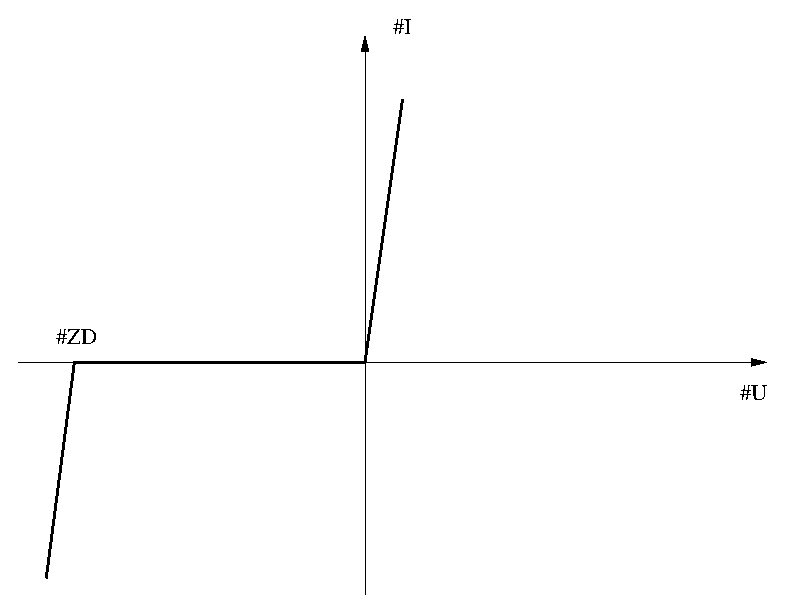
\includegraphics[width=0.4\textwidth]{pyx/zenerdiode.eps}
 \end{center}
 \label{zenerdiode}
 \caption{Kennlinie einer Zenerdiode}
\end{figure}

\section{Kirchhoffsche Gesetze}

\index{Kirchhoffsche Gesetze}

\subsection{Knotengleichungen}

\index{Knotengleichung}

Die Summe aller in einem Knotenpunkt zusammenlaufenden Str"omen ist Null.

\begin{displaymath}
	\sum^n_{i=1}I_i=0
\end{displaymath}

Anders ausgedr"uckt: Die Summe der zum Knoten hineinfliessenden Str"ome ist gleich der Summe der abfliessenden Str"ome.

\subsection{Maschengesetz}

\index{Maschengesetz}

Die Summe aller Spannungen in einer Masche ist Null.

\begin{displaymath}
	\sum^n_{i=1}U_i=0
\end{displaymath}

\section{Serieschaltung von Zweipolen}
\index{Serieschaltung}

In Serie geschaltete Bauelemente sind vom \textit{selben} Strom durchflossen.\\

\index{Serieschaltung}

\subsection{Widerst"ande}
\index{Widerstand, ohm'scher}

\begin{displaymath}
	U=IR_{Serie}
\end{displaymath}
\begin{displaymath}
	R_{Serie}=\sum^n_{i=1}R_i
\end{displaymath}

\index{Spannungsteiler}
Diese Schaltung wird auch als \textit{Spannungsteiler} bezeichnet.

\subsubsection{Spannungsteilerregel}

\begin{figure}[hbt]
 \input Figs/spannungsteiler
 \centerline{\box\graph}
 \caption{Spannungsteiler}
 \label{spannungsteiler}
\end{figure}

Werden zwei Widerst"ande vom selbem Strom durchflossen, so gilt:
\begin{displaymath}
	I = \frac{U_1}{R_1}=\frac{U_2}{R_2}=\frac{U}{R_1+R_2}
\end{displaymath}

Daraus folgt die die Spannungsteilerregel:
\begin{displaymath}
	\frac{U_1}{U_2}=\frac{R_1}{R_2};\quad \frac{U_1}{U}=\frac{R_1}{R_1+R_2};\quad \frac{U_2}{U}=\frac{R_2}{R_1+R_2}
\end{displaymath}

In einer Reihenschaltung sind die Spannungsabf"alle proportional zu den Widerstandswerten, an denen sie abfallen. Dies gilt sinngem"ass auch f"ur Serieschaltungen von mehr als zwei Widerst"anden.\\

Im Allgemeinen:

\begin{displaymath}
	U_k=R_k I_{Serie}=R_k U_{Serie} / R_{Serie} = U_{Serie}\frac{R_k}{\sum^n_{i=1}R_i}
\end{displaymath}

\subsection{ideale Strom- und Spannungsquellen}
\index{Stromquelle, ideale}
\index{Spannungsquelle, ideale}

Serieschaltung idealer Spannungsquellen

\begin{displaymath}
	U_{serie\:q}=\sum^n_{i=1}U_{i\:q}
\end{displaymath}

Eine Serieschaltung idealer Stromquellen mit unterschiedlichen Quellenstr"omen ist verboten.


\section{Parallelschaltung von Zweipolen}

\index{Parallelschaltung}

Parallel geschaltete Bauelemente liegen an derselben Spannung.

\subsection{Widerst"ande}
\index{Widerstand, ohm'scher}

\begin{displaymath}
	I=U\frac{1}{R_{ges}}
\end{displaymath}
\begin{displaymath}
	\frac{1}{R_{ges}}=\sum^n_{i=1}\frac{1}{R_i}
\end{displaymath}

Die Spannung "uber allen Widerst"anden ist gleich.\\

F"ur zwei Widerst"ande $R_1, R_2$ ergibt sich die praktische Formel
\begin{displaymath}
	R_{ges} = \frac{R_1 \cdotp R_2}{R_1 + R_2}
\end{displaymath}

Diese Schaltung wird auch als \textit{Stromteiler} bezeichnet.
\index{Stromteiler}

\subsubsection{Stromteilerregel}

\begin{figure}[hbt]
 \input Figs/stromteilerregel
 \centerline{\box\graph}
 \caption{Stromteiler}
 \label{stromteiler}
\end{figure}

Liegen zwei Leitwerte bzw. Widerst"ande an derselben Spannung, so gilt:

\begin{displaymath}
	U=\frac{I_1}{G_1}=\frac{I_2}{G_2}=\frac{1}{G_1+G_2}
\end{displaymath}

Daraus folgt die Stromteilerregel:
\begin{displaymath}
	\frac{I_1}{I_2}=\frac{G_1}{G_2};\qquad \frac{I_1}{I}=\frac{G_1}{G_1+G_2};\qquad \frac{I_2}{I}=\frac{G_2}{G_1+G_2}
\end{displaymath}

In einer Parallelschaltung sind die Str"ome proportional zu den Leitwerten, durch die sie fliessen. Dies gilt sinngem"ass auch f"ur Parallelschaltungen von mehr anls zwei Leitwerten.\\

Ersetzt man die Leitwerte durch Widerst"ande, so lautet die Stromteilerregel:
\begin{displaymath}
	\frac{I_1}{I_2}=\frac{R_2}{R_1};\qquad \frac{I_1}{I}=\frac{R_2}{R_1+R_2};\qquad \frac{I_2}{I}=\frac{R_1}{R_1+R_2}
\end{displaymath}

Die Teilstr"ome verhalten sich reziprok zu den Widerstandswerten. Ein Teilstrom verh"alt sich zum Gesamtstrom wie der von diesem Teilstrom \textit{nicht} durchflossene Widerstand zu der Summe der Widerst"ande.\\

Im Allgemeinen:
\begin{displaymath}
	I_k = G_k U_{parallel} = G_k I_{parallel} / G_{parallel} = I_{parallel}\frac{G_k}{\sum^n_{i=1}G_i}
\end{displaymath}

\subsection{ideale Strom- und Spannungsquellen}
\index{Stromquelle, ideale}
\index{Spannungsquelle, ideale}

Parallelschaltung idealer Stromquellen

\begin{displaymath}
	I_{parallel\: q}=\sum^n_{i=1}I_{i\: q}
\end{displaymath}

Eine Parallelschaltung idealer Spannungsquellen mit unterschiedlichen Quellenspannungen ist verboten.

\section{Stern-Dreieck Umwandlung}

\index{Stern-Dreieck Umwandlung}

\begin{figure}[hbt]
 \input Figs/stern_dreieck
 \centerline{\box\graph}
 \caption{Links: Dreiecksschaltung, rechts: Sternschaltung}
 \label{stern_dreieck}
\end{figure}

\begin{figure}[hbt]
 \input Figs/stern_dreieck2
 \centerline{\box\graph}
 \caption{Links: $\pi$-Schaltung, rechts: T-Schaltung}
 \label{stern_dreieck2}
\end{figure}

\subsection{Stern (bzw. T) - Dreieck (bzw. $\pi$ Umwandlung)}

\begin{displaymath}
	R_a = \frac{R_1R_2+R_2R_3+R_3R_1}{R_1}
\end{displaymath}
\begin{displaymath}
	R_b = \frac{R_1R_2+R_2R_3+R_3R_1}{R_2}
\end{displaymath}
\begin{displaymath}
	R_c = \frac{R_1R_2+R_2R_3+R_3R_1}{R_3}
\end{displaymath}

\subsection{Dreieck (bzw. $\pi$) - Stern (bzw. T) Umwandlung}

\begin{displaymath}
	R_1 = \frac{R_bR_c}{R_a+R_b+R_c}
\end{displaymath}
\begin{displaymath}
	R_2 = \frac{R_cR_a}{R_a+R_b+R_c}
\end{displaymath}
\begin{displaymath}
	R_3 = \frac{R_aR_b}{R_a+R_b+R_c}
\end{displaymath}

\subsection{Beispiel einer Stern - Dreieck Umwandlung}

\begin{figure}[hbt]
 \input Figs/stern_dreieck_bsp
 \centerline{\box\graph}
 \caption{Beispielschaltung}
\end{figure}

Nach einer Stern - Dreieck Transformation sieht die Schaltung folgendermassen aus.
\begin{figure}[hbt]
 \input Figs/stern_dreieck_bsp2
 \centerline{\box\graph}
 \caption{Transformierte Beispielschaltung}
\end{figure}

Man kann nun mit den Formeln f"ur die Stern- Dreiecksumwandlung die Widerst"ande $R_a, R_b, R_c$ berechnen. Danach kann man die Str"ome durch die Dreick- Widerst"ande berechnen:
\begin{displaymath}
	I_a = \frac{U_2}{R_a}, \qquad I_b = \frac{U_1}{R_b}, \qquad I_c = \frac{U_2 - U_1}{R_c}
\end{displaymath}

Und damit kann man die Str"ome durch die urspr"unglichen Widerst"ande berechnen:
\begin{displaymath}
	I_1 = I_b - I_c, \qquad I_2 = I_a + I_c, \qquad I_3 = -(I_a + I_b)
\end{displaymath}


\section{Th\'evenin, Norton und Quellenumwandlung}

\index{Th\'evenin}
\index{Norton}
\index{Quellenumwandlung}

Wie bereits in ~(\ref{quellenumwandlung_text}) gesehen kann jeder verlustbehaftete, lineare Zweipol entweder als Parallelschaltung einer idealen Stromquelle mit einem Leitwert oder als Serieschaltung einer idealen Spannungsquelle mit einem Widerstand betrachtet werden. Jeder lineare (bzw. linearisierte), verlustbehaftete Zweipol kann also durch eine Stromquellenersatzschaltung oder eine Spannungsquellenersatzschaltung dargestellt werden.\\

Ebenso sieht jedes lineare Netzwerk mit nur zwei Anschlussklemmen von aussen gesehen wie ein linearer Zweipol aus und kann demzufolge durch eine verlustbehaftete Strom-\index{Stromquelle, verlustbehaftete} (Satz von Norton) oder Spannungsquelle \index{Spannungsquelle, verlustbehaftete} (Satz von Th\'evenin) ersetzt werden.

\begin{figure}[hbt]
 \input Figs/thevenin_norton
 \centerline{\box\graph}
 \caption{Prinzipbeispiel f\"ur die Umwandlung einer Schaltung in eine Th\'evenin und in eine Norton \"Aquivalenz}
 \label{thevenin_norton_fig}
\end{figure}

Die Stromquellenersatzschaltung ist von Vorteil, wenn der betreffende Zweipol mit anderen parallel geschaltet, umgekehrt die Spannungsquellenersatzschaltung von Vorteil, wenn der betreffende Zweipol in Serie mit anderen Zweipolen geschaltet ist.\\

Weil Stromquelle (mit Innenleitwert \index{Innenleitwert}) und Spannungsquelle (mit Innenwiderstand \index{Innenwiderstand}) von aussen ununterscheidbar sind, lassen sie sich auch ineinander umformen. Es gilt:\\

\begin{displaymath}
	I_N=\frac{U_T}{R_i} \mbox{ bzw. } U_T=\frac{I_N}{G_I} \mbox{ wobei } R_i=\frac{1}{G_i}=\frac{U_T}{I_N}
\end{displaymath}

\subsection{Beispiel einer Ersatzschaltung nach Th\'evenin und Norton}

Es soll f"ur die folgende Schaltung eine Ersatzschaltung nach Th\'evenin bzw. Norton gefunden werden.

\begin{figure}[hbt]
 \input Figs/thev_norton_bsp_1
 \centerline{\box\graph}
\end{figure}

Man bestimmt als erstes den Innenwiderstand.\\

\usekomafont{descriptionlabel}{1. Leerlauf: Spannungsteiler}
\normalfont

\begin{figure}[hbt]
 \input Figs/thev_norton_bsp_2
 \centerline{\box\graph}
\end{figure}

F"ur $U_L$ ergibt sich:
\begin{displaymath}
	U_L = 20 V \cdotp \frac{10 \Omega}{10 \Omega + 10 \Omega} = 10 V
\end{displaymath}

\usekomafont{descriptionlabel}{2. Kurzschluss}
\normalfont

\begin{figure}[hbt]
 \input Figs/thev_norton_bsp_3
 \centerline{\box\graph}
\end{figure}

\begin{displaymath}
	I_K = \frac{20 V}{ 10 \Omega} = 2 A
\end{displaymath}

\ \\
Damit ergibt sich f"ur den Innenwiderstand:
\begin{displaymath}
	R_i = \frac{U_L}{I_K} = \frac{10 V}{ 2 A} = 5 \Omega
\end{displaymath}

F"ur die Bestimmung des Innenwiderstandes kann man auch eine alternative Methode benutzen. Dabei setzt man die Quellen auf Null und betrachtet die Schaltung von den Klemmen hinein. Man bestimmt den Widerstand der Schaltung, welcher "aquivalent zum Innenwiderstand $R_i$ ist.\\

Und dadurch f"ur die Ersatzschaltungen:\\

Th\'evenin
\begin{displaymath}
	U_0 = U_L = 10 V, \ R_i= 5 \Omega
\end{displaymath}

Norton
\begin{displaymath}
	I_0 = I_K = 2 A, \ R_i= 5 \Omega
\end{displaymath}

\section{Weitere Vereinfachungen und "Uberlegungen}

\subsection{Spannungsquelle}

Eine ideale Spannungsquelle in Parallel mit einem beliebigen Netzwerk (das aber keine andere Spannungsquelle, insbesondere kein Kurzschluss darstellen darf) wirkt von aussen wie die Spannungsquelle allein ($R_i = 0$). Das Netzwerk spielt dabei keine Rolle. Das geht aus der Definition der idealen Spannungsquelle hervor.

\begin{figure}[hbt]
 \input Figs/vereinfachung_spannungsquelle.tex
 \centerline{\box\graph}
 \caption{Vereinfachungen an einer Spannungsquelle}
\end{figure}

\subsection{Stromquelle}

Eine ideale Stromquelle in Serie mit einem beliebigen Netzwerk (das aber keine andere Stromquelle, insbesondere kein offener Kreis, darstellen darf) wirkt von aussen wie die Stromquelle allein ($R_i = \infty$). Das Netzwerk spielt dabei keine Rolle. Das geht aus der Definition der idealen Stromquelle hervor.

\begin{figure}[hbt]
 \input Figs/vereinfachung_stromquelle.tex
 \centerline{\box\graph}
 \caption{Vereinfachungen an einer Stromquelle}
\end{figure}

\section{Quellen\"uberlagerung, Superpostionsprinzip}

\index{Quellen\"uberlagerung}
\index{Superpositionsprinzip}

Nach dem \textit{Superpositionsprinzip} kann in einem linearen Netzwerk die Wirkung \textit{einer} Ursache unabh\"angig von allen anderen Ursachen und Wirkungen berechnet werden. Die resultierende Wirkung ist dann die Summe aller Einzelwirkungen.\\

F\"ur die Berechnung linearer Netzwerke bedeutet dies, dass zun"achst alle Str\"ome einzeln als Wirkung der einzelnen Spannungs- und Stromquellen berechnet werden. Danach werden die so ermittelten Teilstr\"ome vorzeichenrichtig addiert, um den den resultierenden Strom zu bestimmen. Bei der Berechnung der Teilstr\"ome werden die jeweils \textit{nicht} betrachteten Spannungsquellen durch Kurzschl\"usse ersetzt und die jeweils \textit{nicht} betrachteten Stromquellen herausgenommen.\\

\textit{Beispiel:}\\

\begin{figure}[hbt]
 \input Figs/superposition
 \centerline{\box\graph}
 \caption{L\"osungsverfahren nach dem Superpostionsprinzip}
 \label{superposition_fig}
\end{figure}

Kurzschluss der Spannungsquelle $U_q$ und die Anwendung der Stromteilerregel f\"uhrt zu:

\begin{displaymath}
	I_4'=I_q\frac{R_3+\frac{R_1 R_2}{R_1 + R_2}}{R_4+R_3+\frac{R_1 R_2}{R_1+R_2}}
\end{displaymath}

Herausnehmen der Stromquelle $I_q$ und die Anwendung der Stromteilerregel f\"uhrt zu:

\begin{displaymath}
	I_4 '' = I_1 '' \frac{R_2}{R_2+R_3+R_4} = \frac{U_q}{R_1+\frac{R_2(R_3+R_4)}{R_2+R_3+R_4}}\cdotp\frac{R_2}{R_2+R_3+R_4}
\end{displaymath}

Der Strom $I_4$ berechnet sich dann:
\begin{displaymath}
	I_4=I_4'+I_4''
\end{displaymath}


\section{Systematische Methoden}
\index{Systematische Methoden}

\subsection{Knotenanalyse}
\index{Knotenanalyse}

In der Knotenpotentialanalyse ordnet man jedem Knoten ein Potential zu, wobei \textit{ein} Knoten das Bezugspotential $\varphi = 0$ bekommt.

\begin{enumerate}
	\item Wandle alle Spannungsquellen in Stromquellen um.
	\item Man w"ahlt einen beliebigen Knoten als Bezugsknoten. Es ist empfehlenswert, einen m"oglichst grossen Knoten auszuw"ahlen.
	\item F"ur jeden Knoten werden die sogenannten Knotenspannungen zugeordnet. Die entsprechenden Spannungspfeile beginnen beim betreffenden Knoten und enden beim Bezugsknoten. Sind $M$ Knoten vorhanden, so definiert man $M-1$ Knotenspannungen.
	\item Danach stellt man die voneinander unabh"angigen Knotengleichungen auf, indem man die Str"ome mittels der Potentialdifferenzen, geteilt durch die Widerst"ande, ausdr"uckt ($I_n=\Delta\varphi / R_m$).
	\item Dies ergibt ein Gleichungsssystem mit so vielen Gleichungen, wie unbekannte Potentiale vorhanden sind. In Matrixschreibweise:
		\begin{displaymath}
			\mathbf{G}\mathbf{U}=\mathbf{I}
		\end{displaymath}
		Dabei ist $\mathbf{G}$ die Leitwertmatrix. Diese Matrix ist symmetrisch und enth"alt Summen der Leitwerte der verschiedenen Zweipole. $\mathbf{U}$ enth"alt die Knotenspannungen und $\mathbf{I}$ enth"alt die Stromquellen.
	\item Sind die Knotenspannungen durch Aufl"osen des eben erhaltenen Gleichungssystems berechnet, so erh"alt man die Spannungen "uber den Zweipolen sofort aus der Differenz der Knotenspannungen an den beiden Klemmen des Zweipols.
\end{enumerate}

\subsubsection{Beispiel}

\begin{figure}[hbt]
 \input Figs/knotenmethode
 \centerline{\box\graph}
 \caption{Knotenanalyse}
 \label{knotenanalyse_fig}
\end{figure}

In Abbildung ~(\ref{knotenanalyse_fig}) werden nun alle Spannungsquellen durch Stromquellen ersetzt und die Knoten beschriftet dadurch ergibt sich Abbildung ~(\ref{knotenanalyse2_fig}).

\begin{figure}[hbt]
 \input Figs/knotenmethode2
 \centerline{\box\graph}
 \caption{Knotenanalyse}
 \label{knotenanalyse2_fig}
\end{figure}

Nun stellt man die Gleichungen f"ur die verschiedenen Knoten auf:

\begin{description}
	\item[$U_1$:]
	\begin{eqnarray}
		I_1 - I_2 - I_4 &								= &	-I_6 \nonumber\\
		-\frac{U_1}{2\Omega} - \frac{U_1-U_2}{10\Omega} - \frac{U_1}{5\Omega} &		= &	-5 \nonumber
	\end{eqnarray}
	\item[$U_2$:]
	\begin{eqnarray}
		I_2 - I_8 - I_5 &								= &	I_7 \nonumber\\
		\frac{U_1-U_2}{10\Omega} - \frac{U_2}{2\Omega} - \frac{U_2}{4\Omega} &		= &	25 \nonumber
	\end{eqnarray}
\end{description}

In Matrixschreibweise:

\begin{displaymath}
	\left (
		\begin{array}{cc}
			-\frac{1}{2} - \frac{1}{10} - \frac{1}{5} &		\frac{1}{10}\\
			\frac{1}{10} &						-\frac{1}{10} - \frac{1}{2} - \frac{1}{4}\\
		\end{array}
	\right ) 
	\left (
		\begin{array}{c}
			U_1\\
			U_2
		\end{array}
	\right ) =
	\left (
		\begin{array}{c}
			-5\\
			25
		\end{array}
	\right )
\end{displaymath}

\subsection{Maschenanalyse}
\index{Maschenanalyse}

\begin{enumerate}
	\item Man wandelt alle Stromquellen in Spannungsquellen um.
	\item Bei der Methode der Maschengleichungen definieren wir Maschenstr"ome und notieren f"ur diese die Maschengleichungen. Maschenstr"ome sind in einer Masche zirkulierende Str"ome.\\
	Das Auffinden von unabh"angigen Maschen ist etwas schwieriger als das Auffinden unabh"angiger Knoten bei der Knotenanalyse. Man kann systematisch Maschen solange erzeugen, bis jeder Zweipol zu mindestens einer Masche geh"ort und muss dabei lediglich beachten, dass jede neue Masche einen zuvor noch nicht ber"ucksichtigten Zweipol enth"alt, nat"urlich versucht man m"oglichst kleine Maschen zu w"ahlen.
	\item Man notiert nun die Maschengleichungen, in denen die Spannungen "uber idealen Spannungsquellen bekannt sind und die Spannungen "uber Widerst"anden $R_k$ durch $I_k=U_k/R_k$ ersetzt werden
	\item Man ersetzt die Zweipolstr"ome durch die Maschenstr"ome und erh"alt die Matrizengleichung
		\begin{displaymath}
			\mathbf{R}\mathbf{I}=\mathbf{U}
		\end{displaymath}
	Dabei ist $\mathbf{R}$ die symmetrische Widerstandsmatrix. Die Vektoren $\mathbf{I}$ und $\mathbf{U}$ enthalten die Maschenstr"ome und die Quellenspannungen.
	\item Gleichungssystem aufl"osen.
	\item Die unbekannten Str"ome in den Zweipolen werden aus den Maschenstr"omen bestimmt. Dabei werden alle Maschenstr"ome aufsummiert, welche durch den betreffenden Zweipol fliessen
	\item Die unbekannten Spannungen "uber den Widerst"anden werden mit $U_k=R_k/I_k$ berechnet.
\end{enumerate}

\subsubsection{Beispiel}

\begin{figure}[hbt]
 \input Figs/maschenmethode
 \centerline{\box\graph}
 \caption{Maschenanalyse}
 \label{maschenanalyse_fig}
\end{figure}


\begin{description}
	\item[I:]
		\begin{eqnarray}
			U_{2\Omega} + U_{5\Omega} + 25 V &	= &	0 \nonumber \\
			I_1\cdotp 2\Omega +(I_1-I_2)5\Omega &	= &	-25V \nonumber
		\end{eqnarray}
	\item[II:]
		\begin{eqnarray}
			U_{10\Omega} + U_{4\Omega} - 25 V -U_{5\Omega}&		= &	0 \nonumber \\
			I_2\cdotp 10\Omega + (I_2-I_3) 4\Omega - (I_1-I_2) 5\Omega &	= &	25V\nonumber
		\end{eqnarray}
	\item[III:]
		\begin{eqnarray}
			U_{2\Omega} - 50V - U_{4\Omega} &	= &	0 \nonumber \\
			I_{3}\cdotp 2\Omega - (I_2-I_3)4\Omega &	= &	50\nonumber
		\end{eqnarray}
\end{description}

In Matrixschreibweise:

\begin{displaymath}
	\left (
	\begin{array}{ccc}
		7 \Omega &	-5\Omega &	0\\
		-5 \Omega &	19\Omega &	-4\Omega\\
		0 &		-4\Omega &	6\Omega
	\end{array}
	\right ) \left (
	\begin{array}{c}
		I_1\\
		I_2\\
		I_3
	\end{array}
	\right ) = \left (
	\begin{array}{c}
		-25 V\\
		25 V\\
		50 V
	\end{array}
	\right )
\end{displaymath}

\chapter{Schaltvorg"ange}

\section{Kondensatoren und Kapazit"aten}
\index{Kapazit\"at}
\index{Kondensator}

\subsection{"Uberblick}

SI-Einheit: $F$ (Farad); $1F=\frac{As}{V}$\\
\index{Farad}

In der Kapazit"at ist der Strom $i$ proportional zur zeitlichen "Anderung der Spannung $u$.

\begin{displaymath}
	i(t)=C\frac{du}{dt};\qquad u(t)=\frac{1}{C}\int^{t}_{t_0} i(t) dt + U_0;\qquad C= i(t)\frac{dt}{du}
\end{displaymath}

Die Spannung $U_0$ ist die Spannung, die zu Beginn des Integrationsintervalles bereits an der Kapazit"at lag. Speist man eine Kapazit"at mit einem konstanten Strom, so steigt die Spannung linear an.\\

An der Kapazit"at verl"auft die Spannung immer stetig, der Strom kann unstetig sein.\\

F"ur den Zusammenhang von Spannung und Ladungen gilt:
\begin{displaymath}
	U= \frac{Q}{C}
\end{displaymath}

\subsection{Ideale Stromquelle und Kondensator}

Wir betrachten nun den Ladevorgang eines Kondensators, d.h. wir nehmen an, der zun"achst ungeladene Plattenkondensator werde zur Zeit $t=0$ bis zur Zeit $t=T$ an eine ideale Stromquelle $I_0$ angeschlossen.\\

Die Anfangsbedingung lautet $u(0)=0$. Danach ergibt sich ein linearer Spannungsanstieg f"ur $0<t<T$ wegen

\begin{displaymath}
	u(t) = u(0)+\frac{1}{C}\int^t_0 i(t)dt=\frac{1}{C}\int^t_0 I_0dt = \frac{tI_0}{C}
\end{displaymath}

Schliesslich bleibt f"ur $t>T$ die Spannung "uber der Kapazit"at konstant, weil nach $t=T$ kein Strom mehr fliesst. Die Spannung ist dann $u(t)=\frac{I_0T}{C}$.

\subsection{Serieschaltung von R und C an einer Stromquelle}

Anwendung der Maschenregel f"uhrt zu:
\begin{displaymath}
	u = I_0 R + \frac{1}{C}\int I_0 dt
\end{displaymath}

L"osung:
\begin{displaymath}
	u(t) = I_0R + \frac{1}{C}I_0t
\end{displaymath}

Dabei ist $u(t)$ die Spannung "uber $R$ und $C$.

\subsection{Serieschaltung von R und C an einer Spannungsquelle}

"Aquivalent zu einer Stromquelle mit Innenwiderstand.

\begin{figure}[hbt]
 \input Figs/RC_Serie
 \centerline{\box\graph}
 \caption{Serieschaltung von R und C an einer Spannungsquelle}
 \label{RC_Serie}
\end{figure}

Nehmen wir an, dass f"ur $t<0$ der Schalter offen und die Kapazit"at ungeladen sei und dass der Schalter f"ur $t>0$ geschlossen sei.

\begin{displaymath}
	i(t)=\frac{U_0}{R}e^{-\frac{t}{RC}};\qquad u_C(t) = U_0(1-e^{-\frac{t}{RC}});\qquad u_r(t)=U_0e^{-\frac{t}{RC}};\qquad \tau = RC
\end{displaymath}

\begin{figure}[hbt]
 \begin{center}
	\includegraphics[width=0.6\textwidth]{pyx/serie_RC_an_spannungsquelle.eps}
 \end{center}
 \caption{Serieschaltung von R und C an einer Spannungsquelle}
 \label{serie_RC_an_spannungsquelle}
\end{figure}

Eine charakteristische Gr"osse, welche die Geschwindigkeit des Aufladevorgangs beschreibt ist die \textit{Zeitkonstante} \index{Zeitkonstante}

\begin{displaymath}
	\tau=RC
\end{displaymath}

Nachdem die Zeit $t=\tau$ verstrichen ist, ist die Spannung an der Kapazit"at auf $U_0(1-1/e)$ angewachsen.\\

In der Praxis wird der Aufladevorgang immer irgendwann abgebrochen. Wird die Kapazit"at vom Netzwerk getrennt, so dass kein Strom mehr fliessen kann, so bleibt die Spannung konstant.\\

Der Kondensator wird "uber den Widerstand geladen. Da die Spannung "uber dem Kondensator bei diesem Vorgang steigt, wird die Spannung "uber dem Widerstand w"ahrenddessen kleiner. Der Strom ist proportional zur Spannung $u_R$, wird demnach ebenfalls stetig kleiner (siehe Abb. ~\ref{serie_RC_an_spannungsquelle}).

\pagebreak

\subsection{Parallelschaltung von R und C an einer Stromquelle}

\begin{displaymath}
	u(t) = I_0R(1-e^{-\frac{t}{RC}});\qquad i_R(t) = I_0(1-e^{-\frac{t}{RC}});\qquad i_C(t)= I_0\cdotp e^{-\frac{t}{RC}}; \qquad \tau =RC
\end{displaymath}

\begin{figure}[hbt]
 \begin{center}
	\includegraphics[width=0.6\textwidth]{pyx/parallel_RC_an_stromquelle.eps}
 \end{center}
 \caption{Parallelschaltung von R und C an einer Stromquelle}
 \label{parallel_RC_an_stromquelle}
\end{figure}

\subsection{Entladung eines Kondensators}

Betrachtet man aufgeladene, reale Kondensatoren, so stellt man fest, dass diese sich mit der Zeit entladen, man kann reale Kondensatoren mit einer Ersatzschaltung bestehend aus einer Kapazit"at $C$ und einem parallelen Widerstand $R$ approximieren.\\

D.h. wir lassen die Anschl"usse des Kondensators offen.

\begin{figure}[hbt]
 \input Figs/entladung
 \centerline{\box\graph}
 \caption{Ersatzschaltung eines realen Kondensators (mit Innenwiderstand R)}
 \label{schalt_entladung}
\end{figure}

F"ur die Spannung $u$ und den Strom $i_R$ gilt:

\begin{displaymath}
	u(t) = U_0 e^{-\frac{t}{RC}}; \qquad i_R(t)=\frac{u(t)}{R}
\end{displaymath}

Vergleiche den Verlauf der Spannung mit Abbildung ~\ref{serie_RC_an_spannungsquelle}.

\subsection{Parallelschaltung von R und C an einer Spannungsquelle}

Solche Schaltungen f"uhren in der Praxis zur Zerst"orung des Schalters.

\section{Induktivit"at und Spulen}
\index{Induktivit\"at}
\index{Spulen}

\subsection{"Uberblick}

SI-Einheit: $H$ (Henry); $1 H =1\frac{Vs}{A}$\\ \index{Henry}

An der Induktivit"at ist die Spannung $u$ proportional zur zeitlichen "Anderung des Stromes $i$.

\begin{displaymath}
	u=L\frac{di}{dt};\qquad i=\frac{1}{L}\int^{t_1}_{t_0}u(t) dt +I_0;\qquad L=u(t)\frac{dt}{di}
\end{displaymath}

Der Strom $I_0$ ist der Strom, der zu Beginn des Integrationsintervalles bereits floss. Legt man eine konstante Spannung an eine Induktivit"at, so steigt der Strom linear an.\\

In einer Induktivit"at verl"auft der Strom immer stetig, die Spannung kann unstetig sein.\\

Zwischen Induktivit"at und Kapazit"at gilt das Dualit"atsprinzip.\index{Dualit\"atsprinzip}

\subsection{Entladung einer Spule mit Innenwiderstand R}

D.h. wenn die Spulenenden kurzgeschlossen werden.

\begin{displaymath}
	i(t) = I_0 \cdotp e^{-\frac{tR}{L}}
\end{displaymath}

\subsection{Parallelschaltung von R und L an einer Stromquelle}

\begin{displaymath}
	u(t)=I_0R\cdotp e^{-\frac{tR}{L}};\qquad i_L(t)=I_0(1-e^{-\frac{tR}{L}});\qquad i_R(t) = I_0\cdotp e^{-\frac{tR}{L}}; \qquad \tau =\frac{L}{R}
\end{displaymath}

\begin{figure}[hbt]
 \begin{center}
	\includegraphics[width=0.6\textwidth]{pyx/parallel_RL_an_stromquelle.eps}
 \end{center}
 \caption{Parallelschaltung von R und L an einer Stromquelle}
 \label{parallel_RL_an_stromquelle}
\end{figure}

Der Strom $I_0$ fliesst nach dem Umlegen des Schalters zun"achst durch $R$. Der Strom $i_L$ beginnt mit der Steigung $di/dt=I_0R/L$. W"ahrend der Strom $i_L$ steigt, verkleinert sich der Strom $i_R$ bis die Induktivit"at den gesamten Strom $I_0$ "ubernommen hat. Dann ist $u=0$ wegen $i_R=0$ (siehe Abb. ~\ref{parallel_RL_an_stromquelle}).

\subsection{Serieschaltung von R und L an einer Spannungsquelle}

\begin{displaymath}
	i(t) = \frac{U_0}{R}(1-e^{-\frac{tR}{L}});\qquad u_R(t) = U_0(1-e^{-\frac{tR}{L}});\qquad u_L(t) = U_0\cdotp e^{-\frac{tR}{L}};\qquad \tau = \frac{L}{R}
\end{displaymath}

\begin{figure}[hbt]
 \begin{center}
	\includegraphics[width=0.6\textwidth]{pyx/serie_RL_an_spannungsquelle.eps}
 \end{center}
 \caption{Serieschaltung von R und L an einer Spannungsquelle}
 \label{serie_RL_an_spannungsquelle}
\end{figure}

Zum Zeitpunkt $t=0$ liegt die Spannung $u_L=U_0$ an der Induktivit"at. Der Strom $i$ ist zu diesem Zeitpunkt noch Null. Der Strom $i$ beginnt mit der Steigung $di/dt=U_0/L$ gr"osser zu werden. Dadurch wird der Spannungsabfall "uber R zunehmend gr"osser und $u_L$ und $di/dt$ zunehmend kleiner (siehe Abb. ~\ref{serie_RL_an_spannungsquelle}).

\subsection{Serieschaltung von R und L an einer Stromquelle}

$u_L$ w"achst dabei "uber alle Masse und f"uhrt in der Praxis zur Zerst"orung des Schalters.

\subsection{Parallelschaltung von R und L an einer Spannungsquelle}

\begin{displaymath}
	i(t) = \frac{U_0}{R} + \frac{U_0 t}{L}
\end{displaymath}

\section{Physikalische Gr"ossen}

\subsection{Leistung}
\index{Leistung}

SI-Einheit Leistung: W (Watt); 1 W = 1 VA

\textit{momentane} Leistung:
\index{Leistung, momentane}

\begin{displaymath}
	p(t) = u(t)i(t)
\end{displaymath}

Momentanleistung einer Kapazit"at:
\begin{displaymath}
	p(t) = Cu(t)\frac{du}{dt}
\end{displaymath}

Momentanleistung einer Spule:
\begin{displaymath}
	p(t) = Li(t)\frac{di}{dt}
\end{displaymath}

\subsection{Arbeit und Energie}
\index{Arbeit}
\index{Energie}

Die Arbeit/Energie ist das Integral "uber die Leistung

\begin{displaymath}
	w(t) = \int^{t_2}_{t_1} p(t) dt
\end{displaymath}

SI-Einheit Energie: Ws (Wattsekunde); J (Joule)\\

Kapazit"aten und Induktivit"aten speichern die Energie, welche ihnen beim Ladevorgang zugef"uhrt wurde.

\subsubsection{Kapazit"at}

\begin{displaymath}
	w(t_1) = \int_{t_0}^{t_1}u(t)i(t) dt + W_0 = C\int^{t_1}_{t_0} u(t)\frac{du}{dt} dt + W_0=C\frac{u^2(t_1)-u^2(t_2)}{2} + W_0
\end{displaymath}

F"ur Gleichspannung $U$ und $W_0 = 0$ gilt:

\begin{displaymath}
	w(t)=\frac{CU^2(t)}{2}
\end{displaymath}

\subsubsection{Induktivit"at}

\begin{displaymath}
	w(t_1) = \int^{t_1}_{t_0} u(t)i(t) dt + W_0 =  L\int^{t_1}_{t_0} i(t)\frac{di}{dt} dt + W_0 =L\frac{i^2(t_1)-i^2(t_0)}{2} + W_0
\end{displaymath}

F"ur den Gleichstrom $I$ und $W_0 = 0$ gilt:

\begin{displaymath}
	w(t)=\frac{CI^2(t)}{2}
\end{displaymath}

\section{Serieschaltungen}
\index{Serieschaltung}

\subsection{Induktivit"aten}

\begin{displaymath}
	u(t)=L_{ges}\frac{di}{dt}
\end{displaymath}
\begin{displaymath}
	L_{ges}=\sum^n_{i=1}L_i
\end{displaymath}

\subsection{Kapazit"aten}

\begin{displaymath}
	u(t)=\frac{1}{C_{ges}}\int^t_0 idt + U_0
\end{displaymath}
\begin{displaymath}
	\frac{1}{C_{ges}}=\sum^n_{i=1}\frac{1}{C_i}
\end{displaymath}

Die Ladungen Q sind gleich, w"ahrend die Spannungen U umgekehrt proportional ($U_1 = U_2 \cdotp C_2/C_1$) sind.

\section{Parallelschaltungen}
\index{Parallelschaltung}

\subsection{Induktivit"aten}

\begin{displaymath}
	i(t)=\frac{1}{L_{ges}}\int^t_0 u dt + I_0
\end{displaymath}
\begin{displaymath}
	\frac{1}{L_{ges}}=\sum^n_{i=1}\frac{1}{L_i}
\end{displaymath}

\subsection{Kapazit"aten}

\begin{displaymath}
	i(t)=C_{ges}\frac{du}{dt}
\end{displaymath}
\begin{displaymath}
	C_{ges}=\sum^n_{i=1}C_i
\end{displaymath}

Die Ladung Q der Kondensatoren sind umgekehrt proportional, w"ahrend die Spannung U gleich ist.

\chapter{Wechselstrom}
\index{Wechselstrom}

\section{Komplexe Darstellung und Zeiger}
\index{Komplexe Darstelleung}
\index{Zeiger}

Zusammenhang zwischen Kreisfrequenz\index{Kreisfrequenz} und Periode\index{Periode}:

\begin{displaymath}
	\omega = 2\pi / T \qquad \omega = 2\pi f
\end{displaymath}

Sei

\begin{displaymath}
	f(t) = \hat{A}\cos(\omega t +\varphi)
\end{displaymath}

eine harmonische Funktion\index{harmonische Funktion} mit bestimmter Kreisfrequenz $\omega$, Amplitude \index{Amplitude} $\hat{A}$ und Phase \index{Phase} $\varphi$.\\

Diese k"onnen wir mittels Addititionstheorem auf die Form

\begin{displaymath}
	f(t) = a\cos(\omega t) - b\sin(\omega t)
\end{displaymath}

bringen, mit den zwei Amplituden

\begin{displaymath}
	a=\hat{A}\cos\varphi,\qquad b=\hat{A}\sin\varphi
\end{displaymath}

Sind $a$ und $b$ bekannt, so erh"alt man daraus

\begin{displaymath}
	\hat{A} = \sqrt{a^2+b^2},\qquad \varphi = \arctan(b/a)
\end{displaymath}

Wenn man sich das in der 2-dimensionalen xy Ebene vorstellt, so sind $\hat{A}$ und $\varphi$ Polarkoordinaten des Punktes $(a,b)$ in der xy Ebene.\\

Die xy Ebene k"onnen wir aber auch als komplexe Ebene $z=x+jy$ auffassen. In dieser Ebene beschreibt die komplexe Zahl $\underline{C}=a+jb$ die Amplituden $a$ und $b$ unserer harmonischen Funktion und es gilt

\begin{displaymath}
	\hat{A} = \sqrt{\Re(\underline{C})^2+\Im(\underline{C})^2}=|\underline{C}|,\qquad \varphi = \arctan(\frac{\Im(\underline{C})}{\Re(\underline{C})})
\end{displaymath}

Es macht nun Sinn die $f(t)$ folgendermassen zu notieren:

\begin{displaymath}
	f(t) = \Re(\underline{C}e^{j\omega t})
\end{displaymath}


\section{Blind-, Wirk-, und Scheinleistung}

Betrachten wir einen linearen Zweipol, "uber dem die Spannung

\begin{displaymath}
	u(t)=\Re(\underline{U}e^{j\omega t})=\hat{U}\cos(\omega t+\varphi_U)
\end{displaymath}

liegt und durch den der Strom

\begin{displaymath}
	i(t) = \Re(\underline{I}e^{jwt})=\hat{I}\cos(\omega t+\varphi_I)
\end{displaymath}

fliesst. Dabei gilt gem"ass vorhergehendem Abschnitt

\begin{displaymath}
	\hat{U} = \sqrt{\Re(\underline{U})^2+\Im(\underline{U}^2)} = |\underline{U}|, \qquad \varphi_U =\arctan(\Im(\underline{U})/\Re(\underline{U}))
\end{displaymath}
\begin{displaymath}
	\hat{I} = \sqrt{\Re(\underline{I})^2+\Im(\underline{I}^2)} = |\underline{I}|, \qquad \varphi_I =\arctan(\Im(\underline{I})/\Re(\underline{I}))
\end{displaymath}

F"ur den Zeitwert der Leistung des Zweipols gilt also
\begin{displaymath}
	p(t) = \hat{U}\hat{I}\cos(\omega t+\varphi_U)\cos(\omega t+\varphi_I)
\end{displaymath}


\begin{figure}[hbt]
 \begin{center}
	\includegraphics[width=0.6\textwidth]{pyx/leistung.eps}
 \end{center}
 \label{verlauf_leistung}
 \caption{Verlauf von $u(t)$, $i(t)$ und $p(t)$}
\end{figure}


Im Folgenden bezeichnen
\begin{displaymath}
	U_{eff} = \hat{U} / \sqrt{2}; \qquad I_{eff} = \hat{I} / \sqrt{2}
\end{displaymath}

die Effektivwerte von Strom und Spannung \index{Effektivwerte}\\

Die mittlere Leistung \index{Leistung, mittlere} ist definiert als
\begin{displaymath}
	P = \overline{p} = \frac{1}{T} \int^{t + T}_t p(t) dt
\end{displaymath}

\subsection{Scheinleistung}
\index{Scheinleistung}

\begin{displaymath}
	S=U_{eff}I_{eff}
\end{displaymath}

F"ur den Zusammenhang zwischen Schein-, Wirk- und Blindleistung gilt
\begin{displaymath}
	\underline{S} = P + jQ \qquad S = |\underline{S}| = \sqrt{P^2 + Q^2}
\end{displaymath}

\begin{itemize}
	\item Die Wirkleistung ist der Realteil der komplexen Leistung
	\item Die Blindleistung ist der Imagin"arteil der komplexen Leistung
	\item Die Scheinleistung ist der Betrag der komplexen Leistung
\end{itemize}


\subsection{Wirkleistung}
\index{Wirkleistung}

\begin{displaymath}
	P = U_{eff}I_{eff}\cos\varphi, \qquad P = S \cos \varphi
\end{displaymath}

Wobei $\varphi = \varphi_U-\varphi_I$\\

$P$ ist der Mittelwert des Zeitwertes der Wirkleistung. Wirkleistung l"asst sich in andere Formen der Leistung (W"arme usw.) "uberf"uhren.

\subsubsection{Zeitwert der Wirkleistung}
\index{Wirkleistung, Zeitwert}

\begin{displaymath}
	p_W(t) = S \cos(\varphi) [1+\cos 2(\omega t + \varphi_u)]
\end{displaymath}

\subsubsection{Wirkstrom}

\index{Wirkstrom}
Bei der Darstellung eines komplexen Zweipols als Parallel-Ersatzschaltung eines Wirk- und eines Blindwiderstandes kann man den Leistungsfaktor $\cos\varphi$ modellhaft dem Strom zuordnen. Man spricht dann vom \textit{Wirkstrom}.

\begin{displaymath}
	I_w = I \cdotp \cos \varphi
\end{displaymath}

Diese Darstellung ist nur sinnvoll bei Parallelschaltungen.

\subsubsection{Wirkspannung}

\index{Wirkspannung}
Bei der Darstellung eines komplexen Zweipols als Serie-Ersatzschaltung eines Wirk- und eines Blindwiderstandes kann man den Leistungsfaktor $\cos\varphi$ modellhaft der Spannung zuordnen. Man spricht dann von \textit{Wirkspannung}.

\begin{displaymath}
	U_w = U \cdotp \cos \varphi
\end{displaymath}

Diese Darstellung ist nur sinnvoll bei Serieschaltungen.

\subsection{Blindleistung}
\index{Blindleistung}

\begin{displaymath}
	Q = U_{eff}I_{eff}\sin\varphi, \qquad Q = S \sin \varphi
\end{displaymath}

$Q$ ist der Mittelwert des Zeitwertes der Blindleistung. Blindleistung l"asst sich \textit{nicht} in andere Formen der Leistung umwandeln.

\subsubsection{Zeitwert der Blindleistung}
\index{Blindleistung, Zeitwert}

\begin{displaymath}
	p_b(t) = S\sin(\varphi)[\sin 2(\omega t + \varphi_u)]
\end{displaymath}

\subsubsection{Blindstrom}

\index{Blindstrom}
Bei der Darstellung eines komplexen Zweipols als Parallel-Ersatzschaltung eines Wirk- und eines Blindwiderstandes kann man den Leistungsfaktor $\sin\varphi$ modellhaft dem Strom zuordnen. Man spricht dann vom \textit{Blindstrom}.

\begin{displaymath}
	I_b =  -I \cdotp \sin \varphi
\end{displaymath}

Diese Darstellung ist nur sinnvoll bei Parallelschaltungen.

\subsubsection{Blindspannung}

\index{Blindspannung}
Bei der Darstellung eines komplexen Zweipols als Serie-Ersatzschaltung eines Wirk- und eines Blindwiderstandes kann man den Leistungsfaktor $\sin\varphi$ modellhaft der Spannung zuordnen. Man spricht dann von \textit{Blindspannung}.

\begin{displaymath}
	U_b = U \cdotp \sin \varphi
\end{displaymath}

Diese Darstellung ist nur sinnvoll bei Serieschaltungen.

\subsection{Bemerkungen}

Wird das Verbraucherpfeilsystem verwendet und ist die Wirkleistung $P$ eines Zweipols positiv, so nimmt der Zweipol im Zeitmittel Energie auf. Die Blindleistung ist ein Mass f"ur die Energiemenge, welche ein Zweipol w"ahrend jeder Schwingungsperiode aufnimmt und wieder abgibt. Wir werden gleich sehen, dass ideale Kapazit"aten und Induktivit"aten Bauelemente sind, deren Wirkleistung Null ist, deren Blindleistung hingegen positiv ist.

\section{Bauelemente}

\subsection{Quellen}

\subsubsection{Spannungsquelle}
\index{Spannungsquelle}

\begin{displaymath}
	u(t) = \Re(\underline{U}e^{j\omega t})
\end{displaymath}

$\underline{U}$ beinhaltet die Amplitude $\hat{U}$ und die Phasenlage zur Zeit $t=0$:

\begin{displaymath}
	\hat{U} = \sqrt{\Re(\underline{U})^2+\Im(\underline{U})^2}=|\underline{U}|, \qquad \varphi_u = \arctan(\frac{\Im(\underline{U})}{\Re(\underline{U})})
\end{displaymath}

Enth"alt das angeschlossene Netzwerk nur lineare Bauteile und Quellen mit derselben Kreisfrequenz $\omega$, so ist auch der Strom der Spannungsquelle harmonisch und es gilt:

\begin{displaymath}
	i(t) = \Re(\underline{I}e^{j\omega t})
\end{displaymath}
\begin{displaymath}
	\hat{I} = \sqrt{\Re(\underline{I})^2+\Im(\underline{I})^2}=|\underline{I}|, \qquad \varphi_u = \arctan(\frac{\Im(\underline{I})}{\Re(\underline{I})})
\end{displaymath}

Je nach Belastung der Spannungsquelle durch das Netzwerk ergeben sich unterschiedliche Str"ome. Damit kann auch die von der Quelle abgegebene Wirkleistung unterschiedlich gross sein. Wird die Quelle nur durch ein Netzwerk mit Ohm'schen Widerst"anden belastet, so wird die abgegebene Wirkleistung positiv und die Blindleistung $Q=0$.

\subsubsection{Stromquelle}
\index{Stromquelle}
F"ur die ideale harmonische Stromquelle gilt das "aquivalente zur Spannungsquelle, nur ist bei diesen $\underline{I}$ gegeben, w"ahrend sich $\underline{U}$ aus der Belastung durch das angeschlossene Netzwerk ergibt.

\subsection{Widerstand}
\index{Widerstand, ohm'scher}

\begin{displaymath}
	U_{eff} = RI_{eff};\qquad \hat{U}=R\hat{I}; \qquad \varphi_U = \varphi_L; \qquad \underline{U}=R\underline{I}
\end{displaymath}

Der Widerstand verbraucht die Leistung

\begin{displaymath}
	P = \hat{U}\hat{I}/2 = U_{eff}I_{eff}=RI_{eff}^2=U_{eff}^2/R
\end{displaymath}

Die Blindleistung des Widerstandes verschwindet weil die Phasendifferenz von Strom und Spannung verschwindet.

\subsection{Kapazit"at}
\index{Kapazit\"at}

\begin{displaymath}
	\underline{I} = j\omega C \underline{U}; \qquad I_{eff} = \omega CU_{eff}; \qquad \hat{I} = \omega C\hat{U}; \qquad \varphi = -\pi/2
\end{displaymath}

Die letzte Gleichung besagt, dass der Strom der Spannung um \textit{$\pi/2$ nachl"auft}.\\

Die Kapazit"at verbraucht keine Wirkleistung:
\begin{displaymath}
	P = 0
\end{displaymath}

Der Betrag der Blindleistung der Kapazit"at ist maximal. Wird eine Kapazit"at an eine ideale Quelle angeschlossen, so pendelt die gesamte Energie zwischen Quelle und Kapazit"at hin und her.

\subsection{Induktivit"at}
\index{Induktivit\"at}

\begin{displaymath}
	\underline{U} = j\omega L \underline{I}; \qquad U_{eff} = \omega LI_{eff}; \qquad \hat{U} = \omega L\hat{I}; \qquad \varphi = +\pi/2
\end{displaymath}

Die letzte Gleichung besagt, dass der Strom der Spannung um \textit{$\pi/2$ vorl"auft}.\\

Die Induktivit"at verbraucht keine Wirkleistung:
\begin{displaymath}
	P = 0
\end{displaymath}

Der Betrag der Blindleistung der Induktivit"at ist maximal. Wird eine Induktivit"at an eine ideale Quelle angeschlossen, so pendelt die gesamte Energie zwischen Quelle und Induktivit"at hin und her.

\section{Impedanz und Admittanz}

\subsection{Impedanz}
\index{Impedanz}
Bei einer Serieschaltung von Widerstand und Induktivit"at summieren sich die Spannungen und wir erhalten
\begin{displaymath}
	\underline{U} = (R+j\omega L)\underline{I}=\underline{Z}\:\underline{I}
\end{displaymath}

Dabei ist $\underline{Z}=R+j\omega L$ die (komplexe) \textit{Impedanz}. Man schreibt auch $\underline{Z}=R+jX$. Dabei bezeichnet $X$ die Reaktanz.\index{Reaktanz}\\

\textit{Bei Serieschaltungen summieren sich die Impedanzen.}

\subsection{Admittanz}
\index{Admittanz}

Die \textit{Admittanz} ist als der Kehrwert der Impedanz definiert

\begin{displaymath}
	\underline{Y} = 1 /\underline{Z}
\end{displaymath}

\textit{Bei Parallelschaltungen summieren sich die Admittanzen.}


\subsection{Impedanz und Admittanz von Bauelementen}

\subsubsection{Widerstand}
\index{Widerstand, ohm'scher}

\begin{displaymath}
	\underline{Z} = R; \qquad \underline{Y}=\frac{1}{R}
\end{displaymath}

\subsubsection{Kapazit"at}
\index{Kapazit\"at}

\begin{displaymath}
	\underline{Z} = \frac{1}{j\omega C}=\frac{-j}{\omega C}; \qquad \underline{Y}=j\omega C
\end{displaymath}

\subsubsection{Induktivit"at}
\index{Induktivit\"at}

\begin{displaymath}
	\underline{Z} = j\omega L; \qquad \underline{Y}=\frac{1}{j\omega L}=\frac{-j}{\omega L}
\end{displaymath}

\section{Spezielle Schaltungen}

\subsection{Schwingkreise}
\index{Schwingkreise}

\subsubsection{Ideale Schwingkreise}

Da die Impedanzen von $L$ und $C$ - je nach Frequenz - die gesamte positive bzw. negative imagin"are Achse "uberstreichen, \textit{verschwindet f"ur jede $LC$ Serieschaltung die Impedanz} bei einer ganz bestimmten Frequenz $\omega_0$. Es gilt

\begin{displaymath}
	j\omega_0 L - j\frac{1}{\omega_0 C} = 0 \qquad \Rightarrow \omega_0 = \frac{1}{\sqrt{LC}}
\end{displaymath}

Wird die Impedanz Null, so wird nat"urlich die Admittanz \textit{unendlich}.\\

Falls man $L$ und $C$ \textit{parallel} schaltet, so wird die \textit{Admittanz} bei dieser Frequenz $\omega_0$ gleich \textit{Null} und daf"ur die \textit{Impedanz unendlich}.

\begin{figure}[hbt]
 \begin{center}
	\includegraphics[width=0.8\textwidth]{pyx/resonanzkreis.eps}
 \end{center}
 \label{verlauf_leistung}
 \caption{Ortskurve des Betrages $|Z|$ der Impedanz $\underline{Z}$. Links: Serie-, Rechts: Parallelschaltung}
\end{figure}

\subsubsection{Reale Schwingkreise}

In der Praxis lassen sich ideale Induktivit"aten bzw. Kapazit"aten nicht realisieren. Reale Spulen und Kondensatoren weisen Ohm'sche Verluste auf, werden also durch Serie- bzw. Parallelschaltungen von Induktivit"aten bzw. Kapazit"aten mit Widerst"anden approximiert. In der N"ahe der Resonanzfrequenz werden die Widerst"ande dominant.\\

Um die Umgebung der Resonanzfrequenz zu analysieren, wird die \textit{Verstimmung} \index{Verstimmung}

\begin{displaymath}
	\eta = \frac{\omega^2-\omega_0^2}{\omega \omega_0}
\end{displaymath}

eingef"uhrt.\\

Wir f"uhren einen Widerstand in Serie- und Parallelschwingkreis ein um den Ohmschen Verlust von Induktivit"at und Kapazit"at Rechnung zu tragen.\\
Um die Qualit"at eines Schwingkreises zu messen, wird die G"ute \index{G\"ute} $Q$ wie folgt definiert:
\begin{displaymath}
	Q = 2\pi (\text{max. Energie in }L \text{ oder } C)/(\text{pro Periode in }R \text{ in W"arme umgesetzte Energie})
\end{displaymath}

Es ergibt sich f"ur den Serieschwingkreis
\begin{displaymath}
	Q_S = \omega_0 L_S / R_S = \frac{\sqrt{L_S / C_S}}{R_S}
\end{displaymath}

und f"ur eine Parallelschaltung
\begin{displaymath}
	Q_P = \omega_0 C_P R_P = R_P \sqrt{C_P / L_P}
\end{displaymath}

\subsubsection{Bestimmen der Resonanzfrequenz}

Um die Resonanzfrequenz einer beliebigen Schaltung zu bestimmen, benutzt man, dass gelten muss:

\begin{displaymath}
	\Im(\underline{Z}) = 0
\end{displaymath}

$\Re(\underline{Z})$ ist irrelevant und Terme welche $\Im(\underline{Z})$ nicht beeinflussen k"onnen schon vorher weggelassen werden.


\subsection{Zweitore - Passive Filter}
\index{Zweitore}
\index{Filter, Passive}

Besteht aus $RLC$ Netzwerken. Um dieses Zweitor zu charakterisieren, betrachten wir die Ausgangsgr"ossen als Funktion der Eingangsgr"ossen und ihre Abh"angigkeit von der Frequenz.\\

Wir gehen davon aus, dass am Eingang eine ideale Spannungsquelle angeschlossen ist und am Ausgang ein Leerlauf besteht ($\underline{I_a}=0$).

\begin{figure}[hbt]
 \input Figs/zweitor
 \centerline{\box\graph}
 \caption{Passives Zweitor bestehend aus zwei Impedanzen mit idealer Spannungsquelle am Eingang mit Leerlauf am Ausgang.}
 \label{zweitor}
\end{figure}

Da alle beteiligten Komponenten lineare Zweipole sind, muss die Ausgangsspannung proportional zur Eingangsspannung sein:

\begin{displaymath}
	\underline{U}_a = \underline{v}\:\underline{U}_e
\end{displaymath}

Dabei ist die komplexe, frequenzabh"angige Gr"osse $\underline{v}$ die \textit{Verst"arkung}\index{Verst\"arkung} oder \textit{"Ubertragungsfunktion}\index{\"Ubertragungsfunktion} des Zweitors. Deren Betrag ergibt den \textit{Amplitudengang}\index{Amplitudengang} und deren Phase den \textit{Phasengang}\index{Phasengang} des Zweitors.\\

Nach der Spannungsteilerregel gilt f"ur Abb. ~\ref{zweitor}:
\begin{equation}
	v = \frac{\underline{U}_a}{\underline{U}_e} = \frac{\underline{Z}_2}{\underline{Z}_1+\underline{Z}_2}
	\label{zweitor_equation}
\end{equation}

\subsubsection{Hochpass}
\index{Hochpass}

Ist $\underline{Z_1}$ in ~\ref{zweitor_equation} eine Kapazit"at und $\underline{Z}_2$ ein Widerstand $R$, so erhalten wir

\begin{displaymath}
	\underline{v} = \frac{\underline{U}_a}{\underline{U}_e} = \frac{R}{\frac{1}{j\omega C}+R}
\end{displaymath}

und somit f"ur den Betrag der Verst"arkung

\begin{displaymath}
	v = |\underline{v}|=\frac{R}{\sqrt{R^2+1/(\omega C)^2}}
\end{displaymath}

und f"ur die Phase

\begin{displaymath}
	\varphi = \arctan \left( \frac{1}{\omega RC} \right)
\end{displaymath}

F"ur tiefe Frequenzen $(\omega \to 0)$ ist die Verst"arkung 0, f"ur hohe Frequenzen $(\omega \to \infty)$ hingegen nahezu 1.

%TODO Graph schoener
\begin{figure}[hbt]
 \begin{center}
 	\includegraphics[width=0.8\textwidth]{pyx/hochpass.eps}
 \end{center}
 \caption{Bodediagramm, Amplitudengang (links) und Phasengang (rechts) eines RC Hochpasses}
 \label{hochpass}
\end{figure}
\index{Bodediagramm}

Die Frequenz $f_{min}=\omega_{min}/2\pi$,  wobei $w_{min}= \frac{1}{RC}$, ist die untere \textit{Grenzfrequenz}. Es gilt

\begin{displaymath}
	v_{min} = \frac{1}{\sqrt{2}}
\end{displaymath}

Oberhalb der Grenzfrequenz ist der Betrag der Verst"arkung des RC-Hochpasses n"aherungsweise 1.\\

Man benutzt im Normalfall

\begin{displaymath}
	v^{\ast} = 20 \cdotp \lg v \quad[\mbox{db}]
\end{displaymath}
\index{Dezibel}

\begin{remark}
Man kann auch einen Hochpass mit $\underline{Z}_1=R$ und $\underline{Z}_2=L$ oder $\underline{Z}_1=C$ und $\underline{Z}_2=L$ erzeugen.
\end{remark}

\subsubsection{Tiefpass}
\index{Tiefpass}

Setzen wir $\underline{Z}_1=R$ und $\underline{Z}_2=C$, so erhalten wir einen $RC$ \textit{Tiefpass}. Hier gilt:

\begin{displaymath}
	\underline{v} = \frac{1}{1+j\omega RC}
\end{displaymath}

und somit f"ur den Betrag der Verst"arkung

\begin{displaymath}
	v = \frac{1}{\sqrt{1+(\omega RC)^2}}
\end{displaymath}

und f"ur die Phase

\begin{displaymath}
	\varphi = -\arctan (\omega RC)
\end{displaymath}

und die obere Grenzfrequenz
\begin{displaymath}
	\omega_{max} = 2\pi f_{max} =\frac{1}{RC}
\end{displaymath}

%TODO Graph schoener
\begin{figure}[hbt]
 \begin{center}
 	\includegraphics[width=0.8\textwidth]{pyx/tiefpass.eps}
 \end{center}
 \caption{Bodediagramm, Amplitudengang (links) und Phasengang (rechts) eines RC Tiefpasses}
 \label{tiefpass}
\end{figure}

\begin{remark}
Man kann auch einen Tiefpass mit $\underline{Z}_1=L$ und $\underline{Z}_2=R$  oder $\underline{Z}_1=L$ und $\underline{Z}_2=C$ erzeugen.
\end{remark}

\section{Ortskurven}
\index{Ortskurven}

Man kann Serie- und Parallelschaltung von Impedanzen bzw. Admittanzen f"ur verschiedene Frequenzen oftmals bequem  grafisch betrachten. Daf"ur verwendet man die komplexe Impedanz- bzw. Admittanzebene, f"ur das Abzeichnen von Zweipolen gelten folgende Regeln:
\begin{enumerate}
	\item F"ur einen \textit{Widerstand} gilt $\underline{Z} = R$. Folglich ist die Ortskurve des Widerstandes in der komplexen Impedanzebene ein einfacher Punkt auf der reellen Achse: Die Impedanz ist frequenzunabh"angig. Dasselbe gilt nat"urlich auch f"ur die Darstellung von Widerstand und Leitwert in der komplexen Admittanzebene.
	\item F"ur eine \textit{Induktivit"at} gilt $\underline{Z} = j \omega L$. Dadurch wird die positive imagin"are Achse der Impedanzebene beschrieben. Als Spezialf"alle erh"alt man $\underline{Z} = 0$ f"ur $\omega = 0$ und $\underline{Z} = j\infty$ f"ur $\omega=\infty$. Auch in der komplexen Admittanzebene ergibt sich aus $\underline{Y}= 1 / (j \omega L) = - j /(\omega L)$ eine gerade Ortskurve, diesmal jedoch die negative imagin"are Achse mit den speziellen Punkten $-j\infty$ f"ur $\omega=0$ und $\underline{Y} = 0$ f"ur $\omega = \infty$.
	\item F"ur die \textit{Kapazit"at} f"allt die Ortskurve in der Impedanz- bzw. Admittanzebene mit der negativen bzw. positiven imagin"aren Achse zusammen.
\end{enumerate}

Impedanzen kann man nun einfach addieren: Einfach die imagin"ar Teile und real Teile zusammenz"ahlen. F"ur die Inversion also das Umwandeln von Impedanz in Admittanz oder umgekehrt wird es etwas komplizierter: Die Inversion ist aber eine konforme Abbildung, d.h. sie ist winkeltreu und Kreise werden in Kreise abgebildet. Ein Spezialfall sind Geraden, welche als Kreise durch $\infty$ angenommen werden.

\begin{figure}[htb]
\begin{center}
\psset{unit=0.5cm}
\begin{pspicture}(-2,-2)(8,6)
 \psaxes[ticks=none, labels=none]{->}(0,0)(-2,-2)(8,6)
 \psline{->}(0,4)(4,4)
 \psline{-}(3.5,4)(8,4)
 \put(8,-0.9){$\Re(\underline{Z})$}
 \put(0.5,5){$\Im(\underline{Z})$}
 \put(-1.8,4){$j10\Omega$}
\end{pspicture}
\begin{pspicture}(-4,-6)(8,2)
 \psaxes[ticks=none, labels=none]{->}(0,0)(-2,-6)(8,2)
 \pswedge(0,-3){3}{270}{90}
 \put(8,-0.9){$\Re(\underline{Y})$}
 \put(0.5,1){$\Im(\underline{Y})$}
 \put(-2.5,-6){$-j0.1 S$}
\end{pspicture}

\end{center}
\caption{Beispiel einer Inversion einer Ortskurve}
\end{figure}

\chapter{Halbleiterschaltungen}
\index{Halbleiterschaltungen}

\section{Diode}
\index{Diode}

Halbleiter bestehen aus einer einfachen pn Struktur, d.h. aus einer p (positiv) und n (negativ) dotierten Halbleiterschicht.

\subsection{Gleichrichterschaltung}
\index{Gleichrichterschaltung}

Die ideale Diode ist ein idealer \textit{Gleichrichter}, d.h. sie l"asst Strom nur in einer Richtung durch.\\

Die wichtigste Anwendung ist die Umwandlung von Wechsel- in Gleichstrom. Nehmen wir an, es stehe eine Wechselspannungsquelle $u_q(t) = \hat{U}_q\sin(\omega t)$ zur Verf"ugung. Ver\-binden wir einen Anschluss der Wechselspannungsquelle mit einer idealen Diode, so erhalten wir am Ausgang der Diode eine zeitlich ver"anderliche Spannung $u(t)$, deren Vorzeichen stets positiv ist. Es gilt:
\begin{displaymath}
	u(t) = u_q(t), \mbox{ falls } u_q(t) > 0 \mbox{ und andernfalls } u(t) = 0
\end{displaymath}

Will man die zeitabh"angigen Anteile unterdr"ucken, so kann man einen Tiefpass nachschalten. Dessen Grenzfrequenz sollte m"oglichst weit unterhalb der Grundfrequenz $\omega$ liegen.

\begin{figure}[hbt]
 \input Figs/einweggleichrichter
 \centerline{\box\graph}
 \caption{Gleichrichtung mit einer Diode D und nachfolgender Gl"attung mit einer Kapazit"at C, Lastwiderstand R.}
 \label{einweggleichrichter}
\end{figure}

Ein Mangel der sogenannten \textit{Einweggleichrichter}\index{Einweggleichrichter} mit einer einzigen Diode ergibt sich aus der Tatsache, dass die Wechselspannung nur w"ahrend der positiven Halbperiode belastet wird. Abhilfe schafft der \textit{Br"uckengleichrichter} \index{Br\"uckengleichrichter} (Abb. ~\ref{brueckengleichrichter}), welcher aus 4 Dioden besteht.

\begin{figure}[hbt]
 \input Figs/brueckengleichrichter
 \centerline{\box\graph}
 \caption{Gleichrichtung mit einem Br"uckengleichrichter bestehend aus 4 Dioden D mit Lastwiderstand R.}
 \label{brueckengleichrichter}
\end{figure}

F"ur den idealen Br"uckengleichrichter gilt:
\begin{displaymath}
	u(t) = |u_q(t)|
\end{displaymath}

\subsection{Logische Schaltungen}
\index{Logische Schaltungen}

Bei der elektronischen Realisierung bin"arer logischer Schaltungen wird meist der logische Wert $1$ durch eine Spannung oberhalb einer bestimmten Schwelle $U_1$ und der logische Wert $0$ durch eine Spannung unterhalb einer bestimmten Schwelle $U_0$ (mit $U_0 < U_1$) beschrieben.\\

Logische Schaltungen lassen sich mit Netzwerken von Schaltern realisieren.

\begin{figure}[hbt]
 \input Figs/oder_schaltung
 \centerline{\box\graph}
 \caption{ODER-Schaltung mit zwei Dioden und einem Widerstand.}
 \label{oder_schaltung}
\end{figure}

F"ur ideale Dioden ergibt sich
\begin{displaymath}
	u = \max(u_1,u_2)
\end{displaymath}

Stellt $u_1$ oder $u_2$ eine logische $1$ dar, d.h. gilt
\begin{displaymath}
	(u_1 > U_1) \mbox{ ODER } (u_2 > U_1)
\end{displaymath}
so wird auch $u > U_1$, also eine logische $1$. Umgekehrt erh"alt man eine logische $0$ wenn an beiden Eing"angen logische Nullen gesetzt sind.

\section{Bipolare Transistoren}
\index{Transistoren, Bipolare}

Bipolar-Transistoren bestehen aus drei Schichten, entweder in der Reihenfolge pnp oder npn. Die beiden "ausseren Schichten werden \textit{Kollektor}\index{Kollektor} bzw. \textit{Emitter}\index{Emitter} genannt, die mittlere Schicht ist die \textit{Basis}\index{Basis}.

\begin{figure}[hbt]
 \input Figs/transistor
 \centerline{\box\graph}
 \caption{pnp- (links) und npn-(rechts) Transistor}
 \label{transistor}
\end{figure}

Im Normalbetrieb wird die Basis-Emitter-Strecke im Durchlass und die Basis-Kollektor-Strecke im Sperrbereich betrieben. Die Basis-Emitterstrecke verh"alt sich daher wie eine Diode in Durchlaufrichtung (die Pfeilrichtung gibt die Diodenrichtung an). Der positive Basisstrom\index{Basisstrom} fliesst beim npn-Transistor in die Basis hinein, beim pnp-Transistor heraus. Fliesst ein Basisstrom, so fallen "uber der Basis-Emitter-Strecke ca. $0.7V$ ab. Dies ist ein gesch"atzter Wert und kann genau bestimmt werden mit
\begin{displaymath}
	I_B = I_S(\exp(U_{BE}/U_T) -1) \qquad U_T \text{ und } I_S \text{ aus Datenblatt}
\end{displaymath}

Der Basisstrom ist der Steuerstrom. Mit ihm steuert man den Kollektorstrom\index{Kollektorstrom}, sofern eine positive Kollektor-Emitterspannung anliegt. Der Kollektorstrom ist dann n"aher\-ungs\-weise proportional zum Basisstrom.\\

Zwischen $I_B$ und $I_C$ herrscht in guter N"aherung Proportionalit"at:
\begin{displaymath}
	I_C = h_{fE} I_B
\end{displaymath}

In Abbildung ~\ref{ausgangskennlinie_transistor} ist die Ausgangskennlinie $I_C = f(U_{CE})$ dargestellt. Man sieht, dass ab einer minimalen Spannung $U_{CE}$ der Kollektorstrom $I_C$ praktisch nicht mehr von $U_{CE}$ abh"angt, sondern nur noch vom Basisstrom $I_B$.

\begin{figure}[hbt]
 \begin{center}
 	\includegraphics[width=0.7\textwidth]{pyx/kennlinie_transistor.eps}
 \end{center}
 \caption{Kennlinienfeld eines Transistors}
 \label{ausgangskennlinie_transistor}
\end{figure}

\subsection{Grosssignal}

Ein einfaches Modell, welches das Verhalten eines bipolaren npn-Transistors bei Gleichstrom (und bei langsamen Vorg"angen) in erster N"aherung beschreibt, ist das folgende

\index{Grosssignal}
\begin{figure}[hbt]
 \input Figs/grosssignal_ersatz
 \centerline{\box\graph}
 \caption{Einfaches Grosssignal-Ersatzschemata des npn bipolaren Transistors. Beim pnp-Transistor sind die Stromrichtungen und die Polarit"aten der Dioden umgekehrt.}
 \label{grosssignal_ersatz}
\end{figure}

Es k"onnen folgende Betriebsarten unterschieden werden:
\begin{description}
	\item[Cutoff-Bereich] Beide Dioden sind gesperrt, insbesondere die Basis-Emitter Diode: $U_{BE}$ ist positiv bei pnp-, negativ bei npn-Transistoren. Es fliesst kein Strom vom Emitter in die Basis und daher fliesst auch kein Kollektorstrom; man befindet sich im Punkt B auf der Kennlinie.
	\item[S"attigungs-Bereich] Beide Dioden sind leitend. Die Kollektor-Emitterspannung kann zwar nicht negativ werden, sie ist aber sehr klein ($\approx 0.3 V$) und man befindet sich im Punkt A. Es gilt
	\begin{displaymath}
		I_C < h_{fE}I_B
	\end{displaymath}
	Ein Teil des Kollektorstromes fliesst durch die Stromquelle, der andere durch die Diode zur Basis.
	\item[Aktiver Bereich] Die Basis-Emitter Diode ist leitend, w"ahrend die Kollektor-Basis Diode gesperrt ist. In diesem Arbeitsbereich funktioniert der Transistor als Ver\-st"arker. Die Diode $D_{BC}$ kann weggelassen werden.
	\begin{figure}[hbt]
	 \input Figs/grosssignal_ersatz_aktiv
	 \centerline{\box\graph}
	 \caption{Ersatzschaltung des npn bipolaren Transistors im aktiven Bereich}
	 \label{grosssignal_ersatz_aktiv}
	\end{figure}	
\end{description}

\subsection{Der Transistor als Schalter}

In dieser Funktionsart wird der Transistor entweder im Cutoff (Transistor ausgeschaltet, Punkt B) oder in der S"attigung (Transistor eingeschaltet, Punkt A) betrieben.

\subsection{Der Transistor als Verst"arker}
\index{Verst\"arker}

Bei jedem Wert des Eingagangsstromes $I_B$ muss der Transistor dabei im aktiven Bereich bleiben. Daf"ur definiert man einen \textit{Arbeitspunkt}\index{Arbeitspunkt}, um den herum die Strom- bzw. Spannungs"anderungen erfolgen.\\

Solange die Eingangsspannungs"anderung an der BE-Diode klein ist (sogenanntes \textit{Klein\-signalverhalten}\index{Kleinsignal}), kann die Kennlinie um den Arbeitspunkt $(I_{CE},U_{CE0})$ herum als ann"aherend linear betrachtet werden und durch ihre Tangente an diesem Punkt be\-schrieben werden.\\

Wir definieren die \textit{differentiellen Kenngr"ossen}:
\begin{displaymath}
	r_{BE} = \left . \frac{\partial U_{BE}}{\partial I_B}\right |_{U_{CE}=const}\approx \frac{U_T}{I_B}
\end{displaymath}

\begin{displaymath}
	r_{CE} = \left . \frac{\partial U_{CE}}{\partial I_C}\right |_{U_{BE}=const}
\end{displaymath}
$r_{CE}$ bezeichnet die Steigung der Ausgangskennlinie im Arbeitspunkt.

\subsubsection{Kleinsignalverhalten}

Da f"ur das \textit{Kleinsignalverhalten} des Transistors ann"ahernd lineare Verh"altnisse vorausgesetzt werden k"onnen, wird oft das folgende Ersatzschaltbild verwendet.

\begin{figure}[hbt]
 \input Figs/kleinsignal_ersatz
 \centerline{\box\graph}
 \caption{Kleinsignalersatzschaltbild des npn-Transistors}
 \label{kleinsignal_ersatz}
\end{figure}

Die Berechnung von Transistorschaltungen vereinfacht sich dadurch wesentlich, weil dank der Linearit"at der Ersatzschaltung das Superpositionsprinzip angewendet werden kann: Quellen k"onnen separat betrachtet werden.

\pagebreak

\subsection{Grundschaltungen mit Bipolartransistoren}

\begin{table}[htb]
\small
\begin{center}
\begin{tabular}{l||c|c|c}
	&					Emitterschaltung &	Kollektorschaltung &	Basisschaltung \\
	\hline \hline Spannungsverst"arkung $V_u$ &	$>1$ &			$\approx 1$ &		$> 1$ \\
	\hline Stromverst"arkung $V_i$ &	$>1$ &			$> 1$ &			$\approx 1$\\
	\hline Eingangswiderstand $r_e$ &	mittel &		sehr hoch &		sehr klein\\
	\hline Ausgangswiderstand $r_a$ &	hoch &			sehr klein &		hoch
\end{tabular}
\end{center}
\normalsize
\caption{Vergleich zwischen den verschiedenen Betriebsarten eines Transistor}
\end{table}

\subsection{Emitterschaltung}

Der Arbeitspunkt kann entweder "uber den Basisstrom $I_B$ oder "uber die Basis-Emitter Spannung $U_{BE}$ festgelegt werden. Hier wird der Fall mit Festlegung von $I_B$ betrachtet.

\begin{figure}[hbt]
 \input Figs/emitterschaltung
 \centerline{\box\graph}
 \caption{Emitterschaltung als Grundbeschaltung eines bipolaren Transistors. Die beiden Kapazit"aten dienen der Ein- bzw. Auskopplung des Wechselspannungssignals. Sie werden "ublicherweise so gross dimensioniert, dass sie bei der Berechnung des Kleinsignalverhaltens weggelassen werden k"onnen.}
 \label{emitterschaltung}
\end{figure}

Die Arbeitspunktgr"ossen werden im folgenden mit Grossbuchstaben und Index 0 ge\-kennzeichnet. Es gilt also
\begin{displaymath}
	I_B = I_{B0} + i_B, \qquad U_{CE} = U_{CE0} + u_{CE} \qquad \mbox{usw.}
\end{displaymath}

\begin{enumerate}
	\item \textbf{Berechnung des Arbeitspunktes}: Die Wechselspannungsquelle wird Null ge\-setzt. Somit sind nur die Gleichstr"ome zu ber"ucksichtigen. Die Kapazit"aten werden als Unterbruch betrachtet. Unter Ber"ucksichtigung des Grosssignal-Ersatz\-schemas erh"alt man folgende Schaltung, wenn man beachtet, dass die Basis-Kollektor Diode sperrt und deshalb in guter N"aherung weg\-gelassen werden kann.
	\begin{figure}[hbt]
	 \input Figs/ersatz_emmiterschaltung
	 \centerline{\box\graph}
	 \caption{Ersatzschaltung f"ur den Gleichstromfall.}
	 \label{ersatz_emitterschaltung}
	\end{figure}

	Weil die Basis-Emitter Diode im Durchlassbereich arbeitet, k"onnen wir in guter N"aherung $U_{BE} = 0.7V$ schreiben und erhalten:
	\begin{displaymath}
		I_{B0} = (U_0 - 0.7V) / R_B
	\end{displaymath}
	Bei vorgegebenen Arbeitspunkt z.B. $I_{B0} = 60 \mu A$ kann diese Gleichung auch nach $R_B$ aufgel"ost werden. Auf diese Weise wird der Widerstand $R_B$, welcher den Basisstrom und damit den Arbeitspunkt festlegt dimensioniert.\\
	
	Die Kollektor-Emitter Spannung ergibt sich aus folgender Spannungsteilerrechnung:
	\begin{displaymath}
		U_{CE0} = U_0 - R_C I_{C0} = U_0 - R_C h_{fE}I_{B0}
	\end{displaymath}
	\item \textbf{Berechnung der Wechselspannungsgr"ossen}: Hier wird die Speise\-spannungs\-quelle $U_0$ Null (= Kurzschluss) gesetzt. Setzen wir f"ur den Transistor die Klein\-signal-Ersatzschaltung ein, so erhalten wir die Ersatzschaltung gem"ass Figur ~\ref{ersatz2_emitterschaltung}.
	\begin{figure}[hbt]
	 \input Figs/ersatz2_emmiterschaltung
	 \centerline{\box\graph}
	 \caption{Ersatzschaltung f"ur den Wechselspannungsfall (Kleinsignalverst"arkung).}
	 \label{ersatz2_emitterschaltung}
	\end{figure}

	F"ur den Eingangskreis sowie die gesteuerte Stromquelle im Ausgangskreis gilt:
	\begin{displaymath}
		i_B = u_1 / r_{BE}, \qquad i_C = h_{fE} i_B, \qquad u_{CE} = -R_C i_C
	\end{displaymath}
	Durch Einsetzen folgt die Ausgangsspannung
	\begin{displaymath}
		u_2 = u_{CE} = - u_1 h_{fE} R_C / r_{BE}
	\end{displaymath}
	Daraus ergibt sich schliesslich die Spannungsverst"arkung
	\begin{displaymath}
		v = u_2 / u_1 = - h_{fE} R_C / r_{BE}
	\end{displaymath}

\end{enumerate}

\subsection{Gegenkopplung}
\index{Gegenkopplung}

Um die Linearit"at einer einzelnen Verst"arkerstufe und die Stabilit"at des Arbeitspunktes zu verbessern, wird gerne ein Teil des Ausgangssignals an den Eingang zur"uckgef"uhrt und zwar so, dass die Phase des zur"uckgef"uhrten Ausgangssignals gegen"uber der Phase des Eingangssignals um 180 Grad verschoben ist. Damit wirkt das r"uckgef"uhrte Ausgangssignal dem Eingangssignal entgegen und vermindert die Verst"arkung; dies wird Gegenkopplung genannt.\\

Um eine Gegenkopplung bei der Emitterschaltung zu bewerkstelligen, ist keine Phasen\-drehung n"otig, da die Ausgangsspannung der Emitterschaltung gegen"uber der Eingangsspannung bereits um 180 Grad phasenverschoben ist. Man kann also lediglich einen Teil der Ausgangsspannung mit einem Spannungsteiler vom Kollektor abnehmen und an die Basis zur"uckf"uhren. Im wesentlichen wird diese sogenannte \textit{Spannungsgegenkopplung} durch einen Widerstand vom Kollektor zur Basis bewerkstelligt.\\

Die Stromgegenkopplung bei der Emitterschaltung besteht aus einem Widerstand $R_E$ zwischen Emitter und Masse.\\

Die Wirkungsweise der Stromgegenkopplung ist die folgende: Nimmt die Eingangsspannung zu, so nimmt der Kollektorstrom und damit der Emitterstrom zu, welcher nahezu gleich dem Kollektorstrom ist. Damit steigt die Spannung "uber $R_E$ und die Basis-Emitter Spannung wird reduziert, weil
\begin{displaymath}
	U_{Ein} = U_{BE} + U_{R_E}
\end{displaymath}
gilt.

\subsection{Kollektorschaltung, Emitterfolger}
\index{Kollktorschaltung}
\index{Emitterfolger}


\begin{figure}[hbt]
 \input Figs/kollektorschaltung
 \centerline{\box\graph}
 \caption{Prinzip der Kollektorschaltung}
 \label{kollektorschaltung}
\end{figure}

Die Spannungsverst"arkung ist ungef"ahr $v = 1$. Interessant ist diese Schaltung wegen ihres hohen Eingangswiderstandes
\begin{displaymath}
	r_e = r_{BE} + h_{fE} R_E
\end{displaymath}

bei relativ niedrigem Ausgangswiderstand f"ur den gilt
\begin{displaymath}
	r_a \approx \frac{r_{BE}+R_i}{h_{fE}}
\end{displaymath}
Wobei $R_i$ der Innenwiderstand der Spannungsquelle ist, die die Kollektorschaltung speist. Man kann die Kollektorschaltung deshalb als Impedanzwandler verwenden.

\subsection{Basisschaltung}
\index{Basisschaltung}

Bei der Basisschaltung liegt die Basis auf Masse. Wie bei der Emitterschaltung wird der Kollektor "uber einen Widerstand mit der Gleichspannungsquelle verbunden. Ausserdem ist $u_{BE}$ - wie bei der Emitterschaltung - die Eingangsspannung. Die Basisschaltung hat auch dieselbe Spannungsverst"arkung wie die Emitterschaltung, die Ausgangsspannung ist jedoch in Phase mit der Eingangsspannung. Der wichtigste Unterschied zur Emitterschaltung ist der geringe Eingangswiderstand.

\section{Operationsverst"arker}
\index{Operationsverst\"arker}

Bei Operationsverst"arkern will man normalerweise sowohl positive als auch negative Signalspannungen verarbeiten k"onnen. Aus diesem Grunde werden Operationsverst"arker normalerweise mit einer positiven und einer negativen Speisespannung \index{Speisespannung} versorgt. Diese Spannungen sind entgegengesetzt gleich und limitieren den Arbeitsbereich.

\begin{figure}[hbt]
 \begin{center}
	\includegraphics[width=0.7\textwidth]{pyx/uebertragungscharakteristik_opamp.eps}
 \end{center}
 \label{uebertragungscharakteristik_opamp}
 \caption{Idealisierte DC-"Ubertragungscharakteristik eines Operationsverst"arkers}
\end{figure}

Verst"arker, deren Spannungsverst"arkung $v$ einen negativen Wert aufweisen nennt man \textit{Invertierer} \index{Invertierer}. Der Operationsverst"arker verf"ugt "uber einen invertierenden und einen nicht invertierenden Eingang. Die Ausgangsspannnung ist proportional zur Differenz der beiden Eingangsspannungen, d.h. der Operationsverst"arker ist ein \textit{Differenz\-ver\-st"arker}\index{Differenzverst\"arker}.

\begin{figure}[hbt]
 \input Figs/opamp
 \centerline{\box\graph}
 \caption{Schaltung eines Operationsverst"arkers.}
 \label{opamp}
\end{figure}

\subsection{Grundlegende "Uberlegungen}

\begin{figure}[hbt]
 \input Figs/opamp2
 \centerline{\box\graph}
 \caption{Klemmenspannungen und -str"ome eines Operationsverst"arkers.}
 \label{opamp2}
\end{figure}

F"ur die folgende Rechnung gehen wir immer davon aus, dass die Str"ome in den Operationsverst"arker hinein fliessen. \\

Zun"achst muss nat"urlich die Ausgangsspannung im Bereich $U_{B^-}\ldots U_{B^+}$ liegen. Damit der OpAmp im linearen Bereich und nicht in der S"attigung arbeitet, muss die Differenz der Eingangsspannungen gen"ugend klein sein, weil f"ur die Ausgangsspannungen
\begin{displaymath}
	u_0 = A(u_2 - u_1)
\end{displaymath}

gilt, wobei die Spannungsverst"arkung ohne externe Beschaltung $A$ sehr gross ist. Normalerweise ist $A$ sogar so gross ($10000$ und mehr), dass man f"ur die Berechnung in guter N"aherung
\begin{displaymath}
	u_2 = u_1
\end{displaymath}
setzen kann.

Da die Eingangswiderst"ande der beiden Eing"ange sehr hoch sind, kann man die Eingangsstr"ome meist vernachl"assigen, d.h.
\begin{displaymath}
	i_2 = i_1 = 0
\end{displaymath}
setzen.\\

Der Eingangswiderstand eines Operationsverst"arker ist unendlich gross, auch kann er als ideale Spannungsquelle angesehen werden, sein Innenwiderstand ist also gleich Null; somit spielt der Lastwiderstand keine Rolle.

\subsection{Vorgehen bei Berechnungen mit einem Operationsverst"arker}

\begin{figure}[htb]
 \input Figs/opamp_vorgehen1
 \centerline{\box\graph}
 \caption{Beispiel f"ur die Vorgehensweise}
\end{figure}

\begin{enumerate}
	\item Eingangsspannungen aufstellen. F"ur das Beispiel m"ussen wir also die Spannung $U_+$ am nicht-invertierenden Eingang bestimmen. Dies tun wir indem wir die Spannungen mit den Str"omen ausdrucken. Was stets zu beachten ist, ist dass kein Strom in den Operationsverst"arker hinein fliesst. F"ur das Beispiel ergibt sich:
	\begin{eqnarray*}
		U_1 &	= &	I_1 \cdotp R_2 + (I_1 + I_2) \cdotp R_2\\
		U_2 &	= &	I_2 \cdotp R_2 + (I_1 + I_2) \cdotp R_2\\
		U_+ &	= &	(I_1 + I_2) R_2 = \frac{U_1 + U_2}{3}
	\end{eqnarray*}
	\item Benutzen der Gleichung $U_1 = U_2$ und der Tatsache, dass kein Strom in den Operationsverst"arker hineinfliesst. Daf"ur benutzt man am Besten eine Ersatzskizze. 
	\begin{figure}[htb]
	 \input Figs/opamp_vorgehen2
	 \centerline{\box\graph}
	 \caption{Ersatzskizze}
	\end{figure}

	Es muss gelten 
	\begin{displaymath}
		I_{i} = I_{o}
	\end{displaymath}
	
	Umgeschrieben
	\begin{displaymath}
		\frac{-U_{+}}{R_1} = \frac{U_+ - U_0}{2 R_1}
	\end{displaymath}

	Daraus kann man jetzt die Ausgangsspannung in Abh"angigkeit der Eingangsspannungen berechnen.
\end{enumerate}

\subsection{Beschalteter Operationsverst"arker}

Meist verwendet man eine \textit{Gegenkopplung}\index{Gegenkopplung}, d.h. das Ausgangssignal wird "uber einen Zweipol oder ein Netzwerk an den invertierenden Eingang zur"uck gef"uhrt. Geschieht die Gegenkopplung "uber einen einfachen Widerstand, so wird mit diesem im wesentlichen die Verst"arkung eingestellt.\\

Bei vielen Anwendungen wird der nicht invertierende Eingang auf Masse gelegt und das Eingangssignal "uber einen Zweipol oder ein Netzwerk dem invertierenden Eingang zugef"uhrt. Dadurch wird die Schaltungsanalyse besonders einfach, weil man dann f"ur den invertierenden Eingang $i_1 = 0$ und $u_1 = 0$ setzen kann und den nicht invertierenden Eingang f"ur die weitere Rechnung ignorieren kann.

\subsection{Invertierender Verst"arker}
\index{Invertierender Verst\"arker}

Setzen wir den nicht invertierenden Eingang auf Masse und f"uhren wir das Eingangssignal dem invertierenden Eingang "uber einen Ohm'schen Widerstand $R_s$ zu, so erhalten wir einen invertierenden Verst"arker mit praktisch frequenzunabh"angiger Verst"arkung. Mit Hilfe eines Gegenkopplungswiderstandes $R_f$ k"onnen wir die Spannungsverst"arkung auf einen nahezu beliebigen Wert einstellen.

\begin{figure}[hbt]
 \input Figs/opamp_invverst
 \centerline{\box\graph}
 \caption{Invertierender Verst"arker}
 \label{opamp_invverst}
\end{figure}

Wegen $i_1 = 0$ gilt offenbar $i_S = -i_f$. Setzen wir das Ohm'sche Gesetz f"ur die beiden Widerst"ande ein, so folgt wegen $u_1 = 0$ sofort
\begin{displaymath}
	v = u_O / u_S = -R_f/R_S
\end{displaymath}

%\begin{figure}[hbt]
% \input Figs/invverst
% \centerline{\box\graph}
% \caption{Hilfsskizze zur Berechnung}
% \label{invverst}
%\end{figure}

F"ur eine analoge Inversion, d.h. Vorzeichenumkehr des Eingangssignals setzt man $R_f = R_S$ und erh"alt mit $v = -1$ sofort $u_O = - u_S$.

\subsection{Nichtinvertierender Verst"arker}
\index{Nichtinvertierender Verst\"arker}

\begin{figure}[hbt]
 \input Figs/opamp_ninvverst
 \centerline{\box\graph}
 \caption{Nicht-invertierender Verst"arker}
 \label{opamp_ninvverst}
\end{figure}

Die Signalspannungsquelle $u_g$ mit dem Innenwiderstand $R_g$ wird mit dem nicht invertierenden Eingang verbunden. Die Spannungsverst"arkung $v$ wird mit einem Gegenkopplungswiderstand $R_f$ vom Ausgang zum invertierenden Eingang eingestellt; den invertierenden Eingang legen wir "uber einen Widerstand $R_S$ auf Masse.

\begin{displaymath}
	v = 1 + \frac{R_f}{R_g}
\end{displaymath}

\subsection{Addierer}
\index{Addierer}

\begin{figure}[hbt]
 \input Figs/opamp_addierer
 \centerline{\box\graph}
 \caption{Addierer}
 \label{opamp_addierer}
\end{figure}

Verbindet man mehrere Eingangsspannungsquellen "uber Widerst"ande mit dem invertierenden Eingang und verwendet man ausserdem dasselbe Schema wie beim invertierenden Verst"arker, so ergibt sich dieselbe Rechnung wie beim invertierenden Verst"arker, wenn man $i_S$ durch die Summe der Eingangsstr"ome ersetzt. Z.B. gilt f"ur drei Eing"ange:
\begin{displaymath}
	i_S = i_1 + i_2 + i_3
\end{displaymath}

Daraus ergibt sich
\begin{displaymath}
	u_O = - R_f \left (\frac{u_1}{R_1}+ \frac{u_2}{R_2}+ \frac{u_3}{R_3} \right )
\end{displaymath}

Setzt man
\begin{displaymath}
	R_1 = R_2 = R_3 = R_f
\end{displaymath}

So wird offenbar die Ausgangsspannung bis auf das Vorzeichen gleich der Summe der Eingangsspannungen. Um das Vorzeichen zu korrigieren, ist also nur noch ein invertierender Verst"arker mit Spannungsverst"arkung $v=-1$ erforderlich. Zur analogen Addition von beliebig vielen Gr"ossen reichen also zwei Operationsverst"arker.

\pagebreak

\subsection{Subtrahierer}
\index{Subtrahierer}

\begin{figure}[htb]
 \input Figs/opamp_sub
 \centerline{\box\graph}
 \caption{Subtrahierer}
 \label{opamp_sub}
\end{figure}

F"ur $R_2 = R_1 = R_3 = R_f$ finden wir
\begin{displaymath}
	u_O = u_2 - u_1
\end{displaymath}

\subsection{Analoge Integration}
\index{Integration, Analoge}

F"ur die Kapazit"at gilt bekannterweise $i = C \partial u / \partial t$. Die Spannung $u$ "uber der Kapazit"at ist somit das Integral "uber den Strom $i$. 

\begin{figure}[hbt]
 \input Figs/opamp_int
 \centerline{\box\graph}
 \caption{Integration}
 \label{opamp_int}
\end{figure}

F"ur $u_O$ ergibt sich, falls der Kondensator zur Zeit $t_0$ ungeladen war:
\begin{displaymath}
	u_O(t) = -\frac{1}{R_S C_f}\int^t_{t_0} u_S(t')dt'
\end{displaymath}

D.h. die Ausgangsspannung ist das mit dem Faktor $-\frac{1}{R_S C_f}$ skalierte Integral der Eingangsspannung. Um das negative Vorzeichen loszuwerden, kann man wieder einen Inverter nachschalten.

\pagebreak

\subsection{Analoge Differentiation}
\index{Differentiation, Analoge}

\begin{figure}[hbt]
 \input Figs/opamp_diff
 \centerline{\box\graph}
 \caption{Differentiation}
 \label{opamp_diff}
\end{figure}

Man findet daf"ur
\begin{displaymath}
	u_O(t) = -C_S R_f \frac{\partial u_S}{\partial t}
\end{displaymath}

\section{Digitale Schaltungen}
\index{Digitale Schaltungen}

\subsection{Inverter}
\index{Inverter}

\begin{figure}[hbt]
 \input Figs/digi_inverter
 \centerline{\box\graph}
 \caption{Einfacher Inverter in RTL Ausf"uhrung}
 \label{digi_inverter}
\end{figure}

Ist die Eingangsspannung $U_1$ kleiner als etwa $0.6V$ bei einem Siliziumtransistor, so sperrt dieser, d.h. der Kollektorstrom wird klein und $U_a$ wird nahezu gleich der Versorgungsspannung, d.h. gross. Ist umgekehrt $U_1$ gross, so leitet der Transistor und $U_a$ wird klein.

\pagebreak

\subsection{NAND und NOR}

Schaltungstechnisch sind die negierten UND und ODER Verkn"upfungen, NAND und NOR, einfach zu realisieren. Daraus kann man alle logischen Verkn"upfungen durch passende Kombination von NAND und NOR erzeugen. 

\subsubsection{NOR}
\index{NOR}
\begin{figure}[hbt]
 \input Figs/digi_nor
 \centerline{\box\graph}
 \caption{Einfacher NOR Gatter in RTL Ausf"uhrung}
 \label{digi_nor}
\end{figure}

Offenbar leitet der Transistor wenn wenigstens eine der beiden Eingangsspannungen hoch ist, so dass die Ausgangsspannung dann tief wird. Die Ausgangsspannung ist nur dann hoch, wenn beide Eing"ange tief sind.

\subsubsection{NAND}
\index{NAND}

\begin{figure}[hbt]
 \input Figs/digi_nand
 \centerline{\box\graph}
 \caption{Einfacher NAND Gatter in RTL Ausf"uhrung}
 \label{digi_nand}
\end{figure}

Ist beispielsweise $U_2$ hoch, so leitet der "uber $R_2$ angesteuerte Transistor. Damit ein Kollektorstrom fliessen kann, muss aber auch der andere Transistor leiten. $U_a$ wird also nur dann tief, wenn beide Eingangsspannungen hoch sind.

\chapter{Leitungen}
\index{Leitungen}

\section{Zweidrahtleitungen}
\index{Zweidrahtleitungen}

\subsection{Leitungsbel"age}
\index{Leitungsbel\"age}

Man versucht die Leitung durch folgende Gr"ossen zu beschreiben, die man im Normalfall numerisch oder experimentell bestimmt:
\begin{displaymath}
	C', \quad G', \quad R', \quad L'
\end{displaymath}

und $z$ bezeichnet den Ort auf der Leitung.

\subsection{Leitungswellen}
\index{Leitungswellen}

Von den sogenannten Telegraphengleichungen\index{Telegraphengleichung} kommt man auf die entkoppleten Gleichungen
\begin{eqnarray}
	\frac{\partial^2 \underline{U}}{\partial z^2} &		= &	(R' G' + j\omega(R'C'+L'G') - \omega^2 L'C') \underline{U} = (R'+j\omega L')(G' + j\omega C')\underline{U} \nonumber \\
	\frac{\partial^2 \underline{I}}{\partial z^2} &		= &	(R' G' + j\omega(R'C'+L'G') - \omega^2 L'C') \underline{I} = (R'+j\omega L')(G' + j\omega C')\underline{I} \nonumber
\end{eqnarray}

Diese Differentialgleichungen zweiter Ordnung haben L"osungen der Form
\begin{displaymath}
	\underline{U}(z) = \underline{U}^+_0 e^{-\gamma z} + \underline{U}^-_0 e^{+\gamma z}; \qquad \underline{I}(z) = \underline{I}^+_0 e^{-\gamma z} + \underline{I}^-_0 e^{+\gamma z}
\end{displaymath}

Dabei ist die komplexe Gr"osse $\gamma = \alpha + j \beta$ die \textit{Fortpflanzungskonstante}\index{Fortpflanzungskonstante}. Wir finden
\begin{displaymath}
	\gamma = \alpha + j \beta = \sqrt{(R'+j\omega L')(G'+j\omega C')}
\end{displaymath}

Der Realteil $\alpha$ wird \textit{D"ampfungskonstante}\index{D\"ampfungskonstante}, der Imagin"arteil $\beta$ \textit{Phasenkonstante}\index{Phasenkonstante} genannt.

\begin{displaymath}
	u(z,t) = \Re(\underline{U}^+_0e^{j\omega t -\gamma z}+\underline{U}^-_0 e^{j\omega t + \gamma z}); \qquad i(z,t) = \Re(\underline{I}^+_0e^{j\omega t -\gamma z}+\underline{I}^-_0 e^{j\omega t + \gamma z})
\end{displaymath}

Die Terme mit positivem oberem Index beschreiben eine Welle, welche sich mit zunehmender Zeit $t$ in \textit{positive} $z$ Richtung ausbreitet sofern $\beta$ positiv ist. W"ahlt man die $z$ Richtung so, dass die $z$ Achse von der Signalquelle zum Verbraucher zeigt, so kennzeichnen die positiven oberen Indices die \textit{hinlaufende Welle}, die negativen Indices hingegen die \textit{r"uckl"aufigen Wellen}. Ist die D"ampfungskonstante positiv, so nehmen die hinlaufenden Wellen exponentiell mit zunehmendem $z$ ab.\\
Die r"uckl"aufigen Wellen breiten sich in $-z$ Richtung aus und zwar mit derselben Phasenkonstanten und demselben D"ampfungsfaktor wie die hinlaufenden Wellen.

\subsection{Phasengeschwindigkeit}
\index{Phasengeschwindigkeit}

Bedingung f"ur Orte gleicher Phase:
\begin{displaymath}
	\beta z = \omega t \mbox{ oder } z = (\omega / \beta) t
\end{displaymath}

Diese Orte bewegen sich mit der \textit{Phasengeschwindigkeit}
\begin{displaymath}
	v_p = \omega / \beta
\end{displaymath}

in $z$ Richtung. Dasselbe gilt auch f"ur die Str"ome.

\subsection{Charakteristische Impedanz $Z_0$}
\index{Charakteristische Impedanz}
\index{Wellenimpedanz}

\begin{displaymath}
	\underline{Z}_0 = \frac{\underline{U}}{\underline{I}} = \sqrt{\frac{R' + j\omega L'}{G' + j\omega C'}}
\end{displaymath}

Dieser Wert hat die Dimension einer Impedanz und ist charakteristisch f"ur jede Zweidrahtleitung. Man nennt $\underline{Z}_0$ deshalb \textit{charakteristische Impedanz} oder \textit{Wellenimpedanz}.\\
F"ur die r"ucklaufende Welle ergibt sich dieselbe charakteristische Impedanz wie f"ur die hinlaufende Welle.

\subsection{Verlustfreie Leitungen}
\index{Leitungen, verlustfreie}

Sind die Leitungsverluste vernachl"assigbar, so kann man $R' = 0$ und $G' = 0$ einsetzen und erh"alt wesentlich vereinfachte Gleichungen. So gilt f"ur die Fortpflanzungskonstante
\begin{displaymath}
	\gamma = j\beta = j\omega \sqrt{L' C'}
\end{displaymath}

Die D"ampfungskonstante $\alpha$ verschwindet also. Die entsprechenden Wellen breiten sich also unged"ampft aus und die Amplituden am Leitungsende sind ebenso gross wie am Leitungsanfang. F"ur die Phasengeschwindigkeit erh"alt man
\begin{displaymath}
	v_p = \omega / \beta = 1 / \sqrt{L'C'}
\end{displaymath}

Auch die charakteristische Impedanz vereinfacht sich:
\begin{displaymath}
	\underline{Z}_0 = \frac{\underline{U}}{\underline{I}} = \sqrt{\frac{L'}{C'}}
\end{displaymath}
Offensichtlich wird diese Gr"osse reell - wie ein Ohm'scher Widerstand.

\subsection{Phasengeschwindigkeit und Wellenl"ange}
\index{Wellenl\"ange}
\index{Phasengeschwindigkeit}

Es gilt der einfache Zusammenhang zwischen Phasenkonstante und Wellenl"ange
\begin{displaymath}
	\lambda = 2\pi / \beta
\end{displaymath}

Da die exakte Berechnung der Wellenl"ange nicht einfach ist, verwendet man f"ur grobe Absch"atzungen die Freiraumwellenl"ange $\lambda_0$, welche sich aus der Lichtgeschwindigkeit (ca. $3\cdotp 10^8$ m/s) gem"ass
\begin{displaymath}
	\lambda_0 = c / f = 2 \pi c / \omega
\end{displaymath}
berechnen l"asst.

\section{Stossstellen und Abschl"usse}
\index{Stossstellen}
\index{Abschl\"usse}

Verbindet man unterschiedliche Leitungen miteinander, so treten vor allem am "Ubergang (Stossstelle) Ph"anomene auf. 

\subsection{Stossstellen von Zweidrahtleitungen}

Werden zwei Leitungen an einer Stossstelle ($z=0$) verbunden und sind die charakteristischen Impedanzen $\underline{Z}_1$ und $\underline{Z}_2$ der beiden Leitungen unterschiedlich, so wird nicht die ganze Welle \textit{transmittiert}\index{transmittiert} sondern es wird auch noch eine Welle \textit{reflektiert}\index{reflektiert}. F"ur den Strom der transmittierten oder der reflektierten Welle in Abh"angigkeit vom Strom der einfallenden Welle gilt:
\begin{eqnarray}
	\underline{I}_2^+(0)&	= &	\underline{T}\:\underline{I}_1^+(0),\mbox{ wobei } \underline{T} = \frac{2\underline{Z}_1}{\underline{Z}_1 + \underline{Z}_2} \qquad \mbox{transmittierte Welle} \nonumber \\
	\underline{I}_1^-(0)&	= &	\underline{\Gamma}\:\underline{I}_1^+(0),\mbox{ wobei } \underline{\Gamma} = \frac{\underline{Z}_2-\underline{Z}_1}{\underline{Z}_1 + \underline{Z}_2}  \qquad \mbox{reflektierte Welle}  \nonumber
\end{eqnarray}

Dabei ist $\underline{T}$ der \textit{Transmissionskoeffizient}\index{Transmissionskoeffizient} und $\underline{\Gamma}$ der \textit{Reflexionskoeffizient}\index{Reflexionskoeffizient}. $\underline{T}= 1$ und $\underline{\Gamma} = 0$ gilt genau dann, wenn die beiden charakteristischen Impedanzen $\underline{Z}_1$ und $\underline{Z}_2$ gleich sind. Ist dies der Fall, so sind die Leitungen \textit{angepasst}\index{angepasst} und es entsteht keine Reflexion an der Stossstelle.\\

Da sich die transmittierten Wellen mit der Fortpflanzungskonstanten $\gamma_2$ in $+z$ Richtung ausbreiten, gilt f"ur diese
\begin{displaymath}
	\underline{I}_2^+(z) = \underline{T}\:\underline{I}_1^+(0)e^{-\gamma_2 z}
\end{displaymath}

Die reflektierten Wellen hingegen breiten sich in $-z$ Richtung aus, so dass
\begin{displaymath}
	\underline{I}_1^-(z) = \underline{\Gamma}\:\underline{I}_1^+(0)e^{+\gamma_1 z}
\end{displaymath}

\subsection{Leitungsabschluss}
\index{Leitungsabschluss}

Im Wechselstromfall nehmen wir an, der Sender k"onne durch eine Spannungsquelle $\underline{U}_q$ mit Impedanz $\underline{Z}_q$ und der Empf"anger durch eine einfache Lastimpedanz $\underline{Z}_L$ dargestellt werden. F"ur die Reflexionskoeffizienten bei der Last bzw. Quelle gilt:
\begin{displaymath}
	\underline{\Gamma}_L = \frac{\underline{Z}_L - \underline{Z}}{\underline{Z}_L + \underline{Z}}, \qquad \underline{\Gamma}_q = \frac{\underline{Z}_q - \underline{Z}}{\underline{Z}_q + \underline{Z}}
\end{displaymath}

wobei $\underline{Z}$ die charakteristische Impedanz der Leitung ist.\\

Damit ergibt sich offenbar an den Leitungsenden keine Reflexion, wenn die Impedanzen \textit{angepasst} sind, d.h. f"ur $\underline{Z}_L = \underline{Z}$ bzw. $\underline{Z}_q = \underline{Z}$.\\

\textit{Totalreflexion}\index{Totalreflexion} tritt auf, wenn $\underline{\Gamma} = -1$ f"ur $\underline{Z}_L = 0$ bzw. $\underline{Z}_q = 0$ (Kurzschluss) oder $\underline{\Gamma} = +1$ f"ur $\underline{Z}_L = \infty$ bzw. $\underline{Z}_q = \infty$ (Leerlauf).\\

F"ur den Strom und die Spannung auf der Leitung gilt nachdem die reflektierte Welle wieder vorbei ist:
\begin{displaymath}
	U = U^+ + \underbrace{\Gamma U^+}_{U^-} \qquad I = I^+ - \underbrace{\Gamma I^+}_{I^-}
\end{displaymath}

\subsection{Eingangsimpedanz}
\index{Eingangsimpedanz}

Betrachten wir eine \underline{verlustfreie} Leitung ($\alpha = 0, \gamma = j\beta$) mit charakteristischer Impedanz $\underline{Z} = R$, welche auf der einen Seite durch eine sinusf"ormige Spannungsquelle angeregt wird und auf der anderen Seite mit einer Impedanz $\underline{Z}_L = R_L$ belastet wird. Ausserdem sei die Leitung eingangsseitig angepasst, d.h. der Innenwiderstand der Quelle sei ebenfalls $R$.

\begin{figure}[hbt]
 \input Figs/eingangsimpedanz
 \centerline{\box\graph}
 \caption{Verlustlose Leitung angeregt durch eine angepasste Wechselspannungsquelle, belastet mit einem beliebigen Widerstand.}
 \label{eingangsimpedanz}
\end{figure}

\begin{displaymath}
	\underline{\Gamma}_L = \Gamma (0) = \frac{R_L - R}{R_L + R}
\end{displaymath}

Die Reflexion am Lastwiderstand erzeugt eine r"uckl"aufige Welle mit $\underline{U}^-, \underline{I}^-$, welche sich der hinauflaufenden Welle mit $\underline{U}^+, \underline{I}^+$ "uberlagert. Damit ergibt sich f"ur die Spannung und den Strom l"angs der Leitung

\begin{eqnarray}
	\underline{U}(z) &	= &	\underline{U}^+ e^{-j\beta z} + \underline{U}^- e^{+j\beta z} = \underline{U}^+(e^{-j\beta z}+\underline{\Gamma}_L e^{+j\beta z}) = \underline{U}^+ e^{-j\beta z}(1+\underline{\Gamma}_L e^{2j\beta z}) \nonumber \\
	\underline{I}(z) &	= &	\frac{\underline{U}^+ e^{-j\beta z} - \underline{U}^- e^{+j\beta z}}{\underline{Z}} = \underline{U}^+\frac{e^{-j\beta z}-\underline{\Gamma}_L e^{+j\beta z}}{\underline{Z}} = \frac{\underline{U}^+}{\underline{Z}} e^{-j\beta z}(1-\underline{\Gamma}_L e^{2j\beta z}) \nonumber
\end{eqnarray}

Am Eingang messen wir die \textit{Eingangsimpedanz}\index{Eingangsimpedanz}
\begin{displaymath}
	\underline{Z}_{in} = \frac{\underline{U}(-l)}{\underline{I}(-l)} = \frac{\underline{U}^+ (e^{+j\beta l}+\underline{\Gamma}_L e^{-j\beta l})}{\underline{I}^+(e^{+j\beta l}- \underline{\Gamma}_L e^{-j\beta l})} = \underline{Z}\frac{e^{+j\beta l}+\underline{\Gamma}_L e^{-j\beta l}}{e^{+j\beta l}- \underline{\Gamma}_L e^{-j\beta l}}
\end{displaymath}

Umgeformt ergibt dies:
\begin{displaymath}
	\underline{Z}_{in} = \underline{Z} \cdotp \frac{\underline{Z}_L + j\underline{Z}\tan (\beta l)}{\underline{Z}+ j\underline{Z}_L \tan (\beta l)}
\end{displaymath}

Die \textit{normalisierte Reaktanz}\index{Reaktanz} ist definiert als:
\begin{displaymath}
	\bar{X}_{in} = -j\frac{\underline{Z}_{in}}{\underline{Z}} = -j\cdotp \frac{\underline{Z}_L+j\underline{Z}\tan (\beta l)}{\underline{Z}+j\underline{Z}_L \tan(\beta l)}
\end{displaymath}

Die \textit{normalisierte Suszeptanz}\index{Suszeptanz} ist definiert als:
\begin{displaymath}
	\bar{B}_{in} = -j\frac{\underline{Z}}{\underline{Z}_{in}} = -j\cdotp \frac{\underline{Z}+j\underline{Z}_L \tan(\beta l)}{\underline{Z}_L+j\underline{Z}\tan (\beta l)}
\end{displaymath}

\subsection{Stehende Wellen}
\index{Stehende Wellen}

F"ur den Betrag der Spannung auf der Welle gilt:
\begin{displaymath}
	|\underline{U}(z)| = | \underline{U}^+||1 + |\underline{\Gamma}_L|e^{j(\Phi-2\beta z)}|
\end{displaymath}

und f"ur den Strom:
\begin{displaymath}
	|\underline{U}(z)| = | \frac{\underline{U}^+}{\underline{Z}} ||1 - |\underline{\Gamma}_L|e^{j(\Phi-2\beta z)}|
\end{displaymath}

Spannungsmaxima l"angs der Leitung treten offenbar dann auf, wenn $e^{j(\Phi - 2\beta z)}=1$ wird und Spannungsminima wenn $e^{j(\Phi - 2\beta z)}=-1$.\\

Aus der Distanz des ersten Spannungsmaxima vom Leitungsende l"asst sich die \textit{Phase} $\Phi$ \textit{des Reflexionsfaktors} ablesen. Ist die Abschlussimpedanz - ebenso wie die Impedanz der Leitung - reell, so wird der Reflexionsfaktor reell und somit $\Phi = 0$ wenn der Reflexionsfaktor positiv ist, und $\Phi = \pi$ wenn der Reflexionsfaktor negativ ist. Damit findet man am also am Leitungsende entweder ein Spannungsmaxima oder ein Spannungsminimum.\\
Aus dem Ort der Spannungsmaxima l"asst sich aber auch die \textit{Wellenl"ange} auf der Leitung ablesen. F"ur die Distanz $d$ benachbarter Maxima (oder Minima) gilt:
\begin{displaymath}
	2\beta d = 2\pi \Rightarrow \lambda = 2d
\end{displaymath}

Bei Totalreflexion ($\Gamma = -1 \mbox{ oder } +1$) ist das Spannungs- und Stromminima $=0$. Es scheint auch so, dass sich die Welle nicht bewegt, man spricht daher von einer \textit{stehenden Welle}.\\

Ist die Leitung ideal abgeschlossen, so existiert keine reflektierte Welle. Die Spannungs- und Strombetr"age l"angs der Leitung sind konstant.\\

Das Verh"altnis von Spannungsmaxima zu Spannungsminima wird definiert\index{SWR} als
\begin{displaymath}
	SWR = \frac{U_{\max}}{U_{\min}} = \frac{1+|\Gamma_L|}{1-|\Gamma_L|}
\end{displaymath}

SWR ist positiv reell und liegt zwischen 1 (idealer Abschluss) und unendlich (Totalreflexion am Leitungsende). Aus SWR findet man den Betrag des Reflexionsfaktors:
\begin{displaymath}
	|\Gamma_L| = \frac{SWR -1}{SWR +1}
\end{displaymath}

\subsection{Mehrfachreflexionen}
\index{Mehrfachreflexion}

Sind an beiden Leitungsenden Fehlanpassungen vorhanden, so ergeben sich Mehrfachreflexionen, d.h. wiederholt hin- und herlaufende Wellen.\\
Die Signale auf Leitungen mit Mehrfachreflexionen k"onnen mit unendlichen Reihen dargestellt werden. Da die Betr"age der Reflexionskoeffizienten kleiner als $1$ sind, nehmen die Werte mit jeder zus"atzlichen Reflexion ab. Oft gen"ugt es, nur wenige Terme zu ber"ucksichtigen, da die Reihen rasch konvergieren, wenn die Leitungen einigermassen gut angepasst sind.

\appendix

\chapter{Einheiten}


\section{Vielfache von Einheiten}

\begin{table}[htb]
	\renewcommand{\arraystretch}{1.3}
	\begin{center}
	\begin{tabular}{lllp{2cm}lll}
		Faktor &	Vorsatz &	Zeichen &	&	Faktor &	Vorsatz &	Zeichen\\ \hline

		$10^3$ &	Kilo &		k &		&	$10^{-3}$ &	Milli &		m\\
		$10^6$ &	Mega &		M &		&	$10^{-6}$ &	Mikro &		$\mu$\\
		$10^9$ &	Giga &		G &		&	$10^{-9}$ &	Nano &		n\\
		$10^{12}$ &	Tera &		T &		&	$10^{-12}$ &	Piko &		p
	\end{tabular}
	\end{center}
	\caption{Vielfache von Einheiten}
\end{table}

\section{Wichtige Einheiten in der Elektrotechnik}
\begin{table}[htb]
	\renewcommand{\arraystretch}{1.3}
	\begin{center}
	\begin{tabular}{lll}
		Einheit f"ur &		Bezeichnung &	Zeichen\\ \hline

		Strom &			Amp\'ere &	A\\
		Spannung &		Volt &		V\\
		Leistung &		Watt &		W\\
		Widerstand &		Ohm &		$\Omega$\\
		Leitwert &		Siemens &	S\\
		Kapazit"at &		Faraday &	F\\
		Induktivit"at &		Henry &		H
	\end{tabular}
	\end{center}
	\caption{Einheiten in der Elektrotechnik}
\end{table}

\chapter{Trigonometrie}

\section{Funktionswerte f"ur einige Winkel}

\begin{displaymath}
\renewcommand{\arraystretch}{1.7}
\begin{array}{l||lllll}
 \alpha &		0 &		\frac{\pi}{6} &		\frac{\pi}{4} &		\frac{\pi}{3} &		\frac{\pi}{2}\\ \hline\hline
 \sin\alpha &		0 &		\frac{1}{2} &		\frac{\sqrt{2}}{2} &	\frac{\sqrt{3}}{2} &	1\\
 \cos\alpha &		1 &		\frac{\sqrt{3}}{2} & 	\frac{\sqrt{2}}{2} &	\frac{1}{2} &		0\\
 \tan\alpha &		0 &		\frac{\sqrt{3}}{3} &	1 &			\sqrt{3} &		-
\end{array}
\end{displaymath}


\section{Trigonometrische Kurven}

\begin{figure}[htb]
	\begin{center}
		\begin{tabular}{lcr}

		\multirow{7}{2.7cm}[0.2cm]{
			\psset{xunit=0.0111cm,yunit=0.75cm}
			\begin{pspicture}(-105,-4.5)(130,4.5)
				\psline[linewidth=1pt]{->}(-90,0)(90,0)
				\psline[linewidth=1pt]{->}(0,-4.5)(0,4.5)
				\psline[linestyle=dotted]%
				  (-90, -4.5)(-90,4.5)\rput(-90,-0.3){-$\frac{\pi}{2}$}
				\psline[linestyle=dotted]%
				  (-45, -4.5)(-45,4.5)\rput(-45,-0.3){-$\frac{\pi}{4}$}
				\psline[linestyle=dotted]%
				  (45, -4.5)(45,4.5)\rput(45,-0.3){$\frac{\pi}{4}$}
				\psline[linestyle=dotted]%
				  (90, -4.5)(90,4.5)\rput(90,-0.3){$\frac{\pi}{2}$}
				\multido{\n=-4+1}{9}{\psline[linestyle=dotted]%
				  (-90,\n)(90,\n)\rput[r](-4,\n){\scriptsize \n}}
				\psplot[plotstyle=curve,linewidth=1.5pt]%
				  {-78}{78}{x sin x cos div}% postscript function
				%\rput[l](-5,1.75){$\mathbf{y}$}
				%\rput[l](105,-.3){$\mathbf{x}$}
				\rput[l](-55,3.3){$y=\tan x$}
			\end{pspicture}
		}
		\\ \\

		& &
			\psset{xunit=0.0111cm,yunit=1cm}
			\begin{pspicture}(-20,-1.25)(410,1.25)
				\psline[linewidth=1pt]{->}(-20,0)(400,0)
				\psline[linewidth=1pt]{->}(0,-1.25)(0,1.25)
				%\multido{\n=+90}{5}{\psline[linestyle=dotted]%
				%  (\n,-1.25)(\n,1.25)\rput(\n,-0.25)%
				%  {\scriptsize \n}}
				\multido{\n=+90}{5}{\psline[linestyle=dotted]%
				  (\n,-1.25)(\n,1.25)}
				\rput(90,-0.25){\small $\frac{\pi}{2}$}
				\rput(180,-0.25){\small $\pi$}
				\rput(270,-0.25){\small $\frac{3 \pi}{2}$}
				\rput(360,-0.25){\small $2 \pi$}

				\multido{\n=-1+1}{3}{\psline[linestyle=dotted]%
				  (0,\n)(405,\n)\rput[r](-4,\n){\scriptsize \n}}
				\psplot[plotstyle=curve,linewidth=1.5pt]%
				  {-20}{400}{x sin}% postscript function
				\rput[l](-5,1.75){$\mathbf{y}$}
				\rput[l](390,-.25){$\mathbf{x}$}
				\rput[l](180,0.75){$y=\sin x$}
			\end{pspicture}
		\\
		\\
		& &
			\psset{xunit=0.0111cm,yunit=1cm}
			\begin{pspicture}(-20,-1.25)(410,1.25)
				\psline[linewidth=1pt]{->}(-20,0)(400,0)
				\psline[linewidth=1pt]{->}(0,-1.25)(0,1.25)
				%\multido{\n=+90}{5}{\psline[linestyle=dotted]%
				%  (\n,-1.25)(\n,1.25)\rput(\n,-0.25)%
				%  {\scriptsize \n}}
				\multido{\n=+90}{5}{\psline[linestyle=dotted]%
				  (\n,-1.25)(\n,1.25)}
				\rput(90,-0.25){\small $\frac{\pi}{2}$}
				\rput(180,-0.25){\small $\pi$}
				\rput(270,-0.25){\small $\frac{3 \pi}{2}$}
				\rput(360,-0.25){\small $2 \pi$}
				\multido{\n=-1+1}{3}{\psline[linestyle=dotted]%
				  (0,\n)(405,\n)\rput[r](-4,\n){\scriptsize \n}}
				\psplot[plotstyle=curve,linewidth=1.5pt]%
				  {-20}{400}{x cos}% postscript function
				\rput[l](-5,1.75){$\mathbf{y}$}
				\rput[l](390,-.25){$\mathbf{x}$}
				\rput[l](180,0.75){$y=\cos x$}
			\end{pspicture}
		\\
		\\
		\end{tabular}
	\end{center}
	\caption{Trigonometrische Kurven}
\end{figure}


\printindex

\end{document}
